\subsection{Open Targets}
\label{subsec:ot}

Open Targets is a large--scale, public--private partnership with the aim of generating an informatics platform that utilises genetic germline, genetic somatic, gene expression, literature, pathway, and drug data to link 18,104 genes and diseases, with the ultimate objective of developing a systematic priorisation of gene--disease associations (GDAs) \cite{ferrero2017}.
\begin{itemize}
    \item Which were the \textbf{targets}? The targets could be a genes, transcripts or proteins defined by standard nomenclature. Which one is this nomenclature? Ensembl? HUGO? I think it is Ensembl for their research
    
    \item Which were the \textbf{diseases}? Diseases were described by the \href{https://goo.gl/YvvC8D}{EFO} \cite{experimentalFactorOntology2010}
    
    \item How they relate phenotypes to diseases? The evidence is described in the \href{https://goo.gl/CNqAqt}{Open Biomedical AssociatioN} (OBAN) representation \cite{sarntivijai2016}. OBAN is an ontology that represents triple-form entities of \texttt{subject--related--to\_object}. For example, an entity \texttt{disease} is the subject, the relationship \texttt{has\_evidence} and the objects could be entities \texttt{phenotypes} plus the source of evidence for that association
    
\end{itemize}

\subsubsection{Data sources}
\label{subsubsec:ot_ds}
% Always in this alphabetic order:
% Affected pathway
% Animal model
% Genetic association
% Somatic association
% Known drug
% Literature text mining
% RNA expression

The information obtained from different public domain databases (see Table \ref{tab:ot_db}) was classified into seven different \texttt{data types}:

\begin{itemize}
    \item \texttt{affected\_pathway}: if the gene is known to be part of a pathway that is affected in disease

    \item \texttt{animal\_model}: if an animal model with a gene knockout or phenotype that manifests in phenotype concordant with human disease
    
    \item \texttt{genetic\_association}: if there are germline mutation with either common disease primarily from GWAS or rare Mendelian disease from sequencing of exons of protein coding genes
    
    \item \texttt{somatic\_association}: if there is somatic mutation in the gene associated with the disease
    
    \item \texttt{known\_drug}: if there is an existing drug that engages the target and is used to treat the disease from \href{https://goo.gl/tJ2wzt}{ChEMBL}
    
    \item \texttt{literature} if a GDA was identified through co-occurrence in full text articles from \href{https://europepmc.org/}{Europe PMC database} \cite{koscielny2016}
    
    \item \texttt{rna\_expression}: if there are significant gene expression changes in appropriate sample comparisons from microarray or RNA-seq experiments as a consequence of the disease
\end{itemize}

\begin{table}[H]
\centering
    \begin{tabular}{c|c|c|c}
      Data source & Data type & \texttt{evidence\_score} \\
      \hline
      
      \href{https://goo.gl/sfm7CC}{Reactome} & Affected pathway &
      Curator score = \{1,0\} \\
      
      \href{https://goo.gl/egMxCH}{PhenoDigm} & Animal Model &
      Similarity score \cite{PhenoDigm2013} \\
      
      \href{https://goo.gl/A4UjA5}{GWAS Catalog} & Genetic association &
      $ FCS^* \cdot sample\_size \cdot p_{value} $ \\
      
      \href{https://goo.gl/Vavb1L}{EVA} & Genetic association & 
      FCS* \\
      
      \href{https://goo.gl/5SiDMj}{UniProt} & Genetic association &
      Curator score = \{0.5,1\} \\
      
      \href{https://goo.gl/qwDPhK}{Gene2Phenotype} & Genetic association &
      Curator score = 1 \\
      
      \href{https://goo.gl/dXL3jQ}{Cancer Gene Census} & Somatic mutation &
      FCS* \\
      
      \href{https://goo.gl/kTWn6z}{IntOGen} & Somatic Mutation &
      Tumor type category score = \{0.25, 0.5, 0.75\}\\
      
      \href{https://goo.gl/tJ2wzt}{ChEMBL} & Known drug & Clinical phase score = \{0.09, 0.1, 0.2, 0.7, 1.0\} \\
      
      \href{https://goo.gl/P3UAc9}{Europe PMC} & Literature text mining & Confidence score \cite{kafkas2017} \\
      
      \href{https://goo.gl/1eQbbs}{Gene Expression Atlas} & RNA expression & $p_{value} \cdot sample\_size \cdot percentile\_rank $ \\
      
      \end{tabular}
\caption{Data sources for GDA information the Open Targets pipeline. The \texttt{evidence\_score} is described in Section \ref{subsubsec:ot_scores}. A more detailed explanation of the \texttt{evidence\_score} is described by Koscielny et al. \cite{koscielny2016} \label{tab:ot_db}}
\end{table}

* FCS means Functional Consequence Score. Available in \href{https://goo.gl/gkvHxK}{Supplementary Table 2. Functional consequence score}

All information in Open Targets is stored in JSON format. An example of the JSON format they use can be viewed in Figure \ref{fig:ot_json}.

\begin{figure}[H]
    \centering
    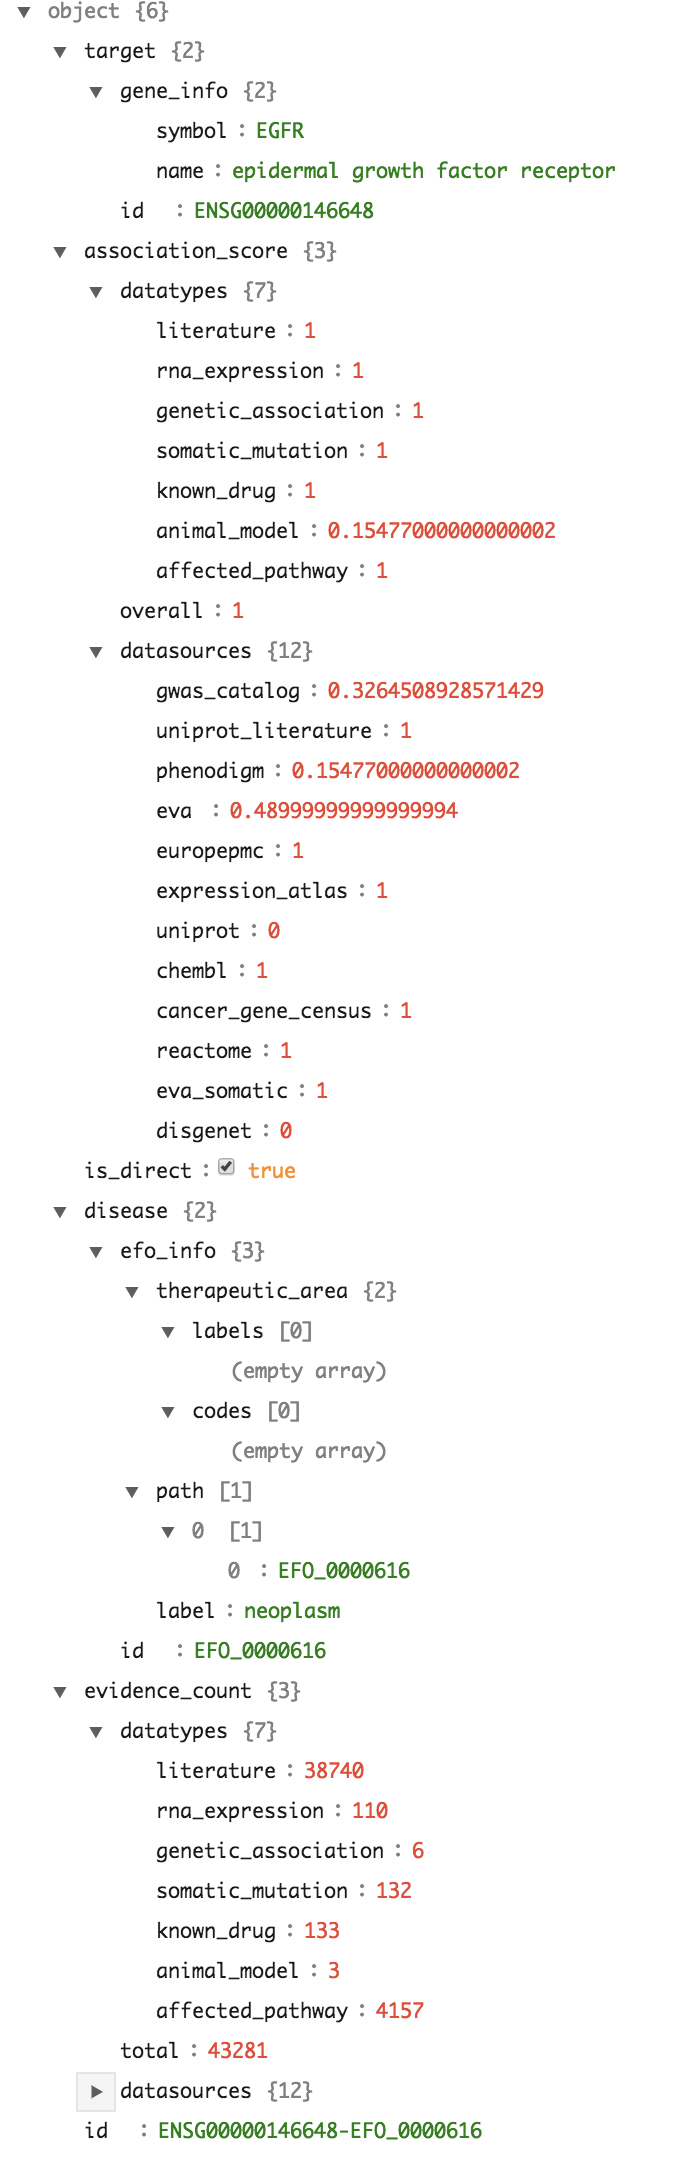
\includegraphics[width=7cm]{pics/ot_json.png}
    \caption{JSON format in Open Targets \label{fig:ot_json}}
\end{figure}

\subsubsection{Scores}
\label{subsubsec:ot_scores}

\begin{itemize}
    \item \texttt{evidence\_score} that attempts to comprise the (i) \texttt{frequency}, (ii) \texttt{magnitude}, and (iii) \texttt{confidence} of GDAs \cite{koscielny2016} in Table \ref{tab:ot_db}. E.g. in a GWAS evidence from GWAS Catalog: the \texttt{frequency} is the sample size, the \texttt{magnitude} is the predicted functional consequence of the variation, and the \texttt{confidence} is the p-value
    
    \item \texttt{data\_source\_score} defined as the \emph{harmonic sum} of all sorted evidence scores in descending order. E.g. in a GWAS evidence from GWAS Catalog: all \texttt{evidence scores} are sorted in descending order and the \texttt{data\_source\_score} is calculated based on the formula below:
    
    $$ S_{1,...i} = S_1 + \frac{S_2}{2^2} + \frac{S_3}{3^2} + ... + \frac{S_i}{i^2}$$
    
    \item \texttt{data\_type\_score} follows a similar approach to the \texttt{data\_source\_score}. It uses the \emph{harmonic sum} to derive a unique score for each of the data types described in Section \ref{subsubsec:ot_ds}. E.g. in a GWAS evidence, the harmonic sum is calculated based on the formula above with the four \texttt{data\_source\_scores} for \texttt{genetic\_association}: GWAS Catalog, EVA, UniProt, and Gene2Phenotype in Table \ref{tab:ot_db}
    
    
    
    \item \texttt{overall\_score} follows the same approach as the \texttt{data\_type\_score} and \texttt{data\_source\_score}
\end{itemize}

Why the harmonic sum? Is there a better score? Idea: use different scores and do a sensitivity analysis

Why they include \texttt{sample\_size}? It is already included in the p-value! The p-value is a measure of uncertainty. The more data, the less uncertainty. The code snippet below in \texttt{Python} will demonstrate it:

\lstinputlisting[language=Python]{data/pval_uncertainty.py}

\subsubsection{Reproduction of pipeline}
Ferrero et al. code in R version 3.3.0 was versioned using GitHub and is available \href{https://goo.gl/C4cSgQ}{elsewhere}.
They defined different sets in the workflow (see Figure \ref{fig:ot_workflow}):
\begin{itemize}
    \item The \texttt{main set} (2016 Apr version) is a \texttt{JSON} file downloaded from the \href{https://goo.gl/BdqKkH}{platform download page} and contains all Open Targets GDAs. Just 5 of the 7 described features in Section \ref{subsubsec:ot_ds} were used: \texttt{affected\_pathway}, \texttt{animal\_model}, \texttt{genetic\_association}, \texttt{rna\_expression} and \texttt{somatic\_mutation}. They removed \texttt{known\_drug} and \texttt{literature}
    
    \item The \texttt{label set} with information on (i) genes and (ii) associated drugs based on PharmaProjects data \cite{pharmaProjects}. Genes with drugs in Preclinical, Clinical Trial Phase I, Clinical Trial Phase II, Clinical Trial Phase III, Pre-registration, Registered, or Launched were considered targets. Failed and Abandoned drugs were ignored. \textbf{Important} The results in this report were obtained using the targets from Cortellis, provided by Guillermo.
    
    \item The \texttt{working set} with all known PharmaProject targets (n=1421) and randomly selected unlabelled (n=1421)
    
    \item The \texttt{prediction set} with the remaining unlabelled genes (n=15262) that was set aside for the prediction of targets
\end{itemize}

Restrictions apply to the availability of the Pharmaprojects data \cite{ferrero2017}. Why did Open Targets used PharmaProjects data if they had \href{https://goo.gl/StJTq2}{ChEMBL} \cite{chembl2014} data as mentioned in Section \ref{subsubsec:ot_ds}?
\begin{itemize}
    \item It covers early stage announcements
    \item It contains more targets with drug annotations (2105 versus 625)
    \item It discriminates between drug development phases: Preclinical, Clinical Trial, Phase I Clinical Trial, Phase II Clinical Trial, Phase III Clinical Trial, Pre-registration, Registered, Launched, Failed, or Abandoned
\end{itemize}


\begin{figure}[H]
    \centering
    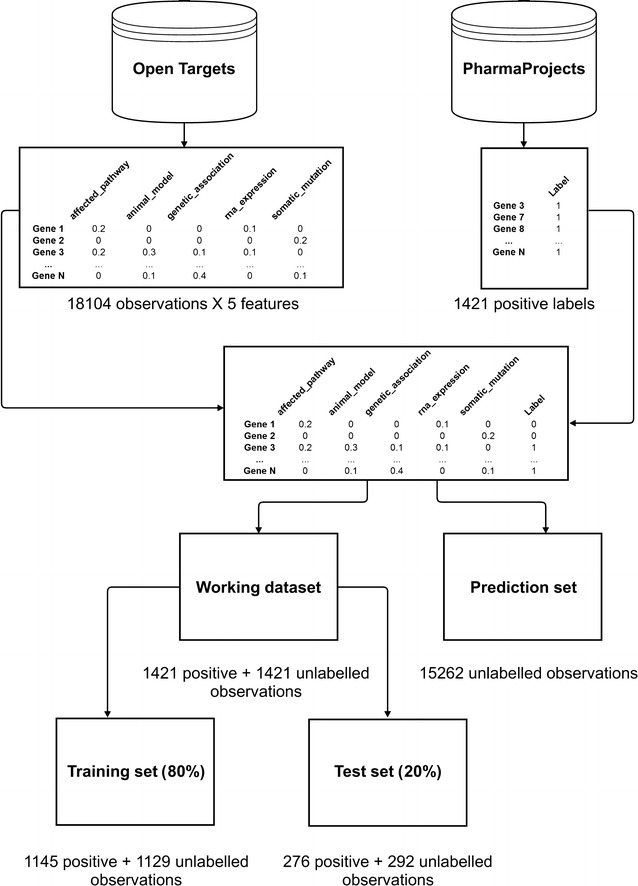
\includegraphics[width=0.7\textwidth]{pics/workflowOpenTargets.jpg}
    \caption{Explanatory workflow for the prediction of therapeutic targets based on GDAs. Observations and features were gathered by Open Targets based on just 5 of the 7 data types from Section \ref{subsubsec:ot_ds} while the labels were collected from Informa Pharmaprojects \cite{pharmaProjects} (my results use Cortellis targets provided by Guillermo). The resulting data matrix was split into a \texttt{working set} (1421 positives and 1421 randomly selected unlabelled) and a \texttt{prediction set} (15262 unlabelled genes). The \texttt{working set}, containing both positive and unlabelled observations, was further split into \texttt{training set} and \texttt{test set} to evaluate the performance of the classifier. The \texttt{prediction set} was kept aside and used to perform predictions once all four classifiers was trained}
    \label{fig:ot_workflow}
\end{figure}

Second, Ferrero et al. \cite{ferrero2017} carried out an exploratory analysis on the \texttt{working set} using two unsupervised methods: principal component analysis (PCA) and t-Stochastic Neighbourhood Embedding (tSNE). PCA and t-SNE results are displayed in Figure \ref{fig:OT_PCA} and Figure \ref{fig:OT_tSNE} respectively.

\begin{figure}[H]
\resizebox{\textwidth}{!}{
    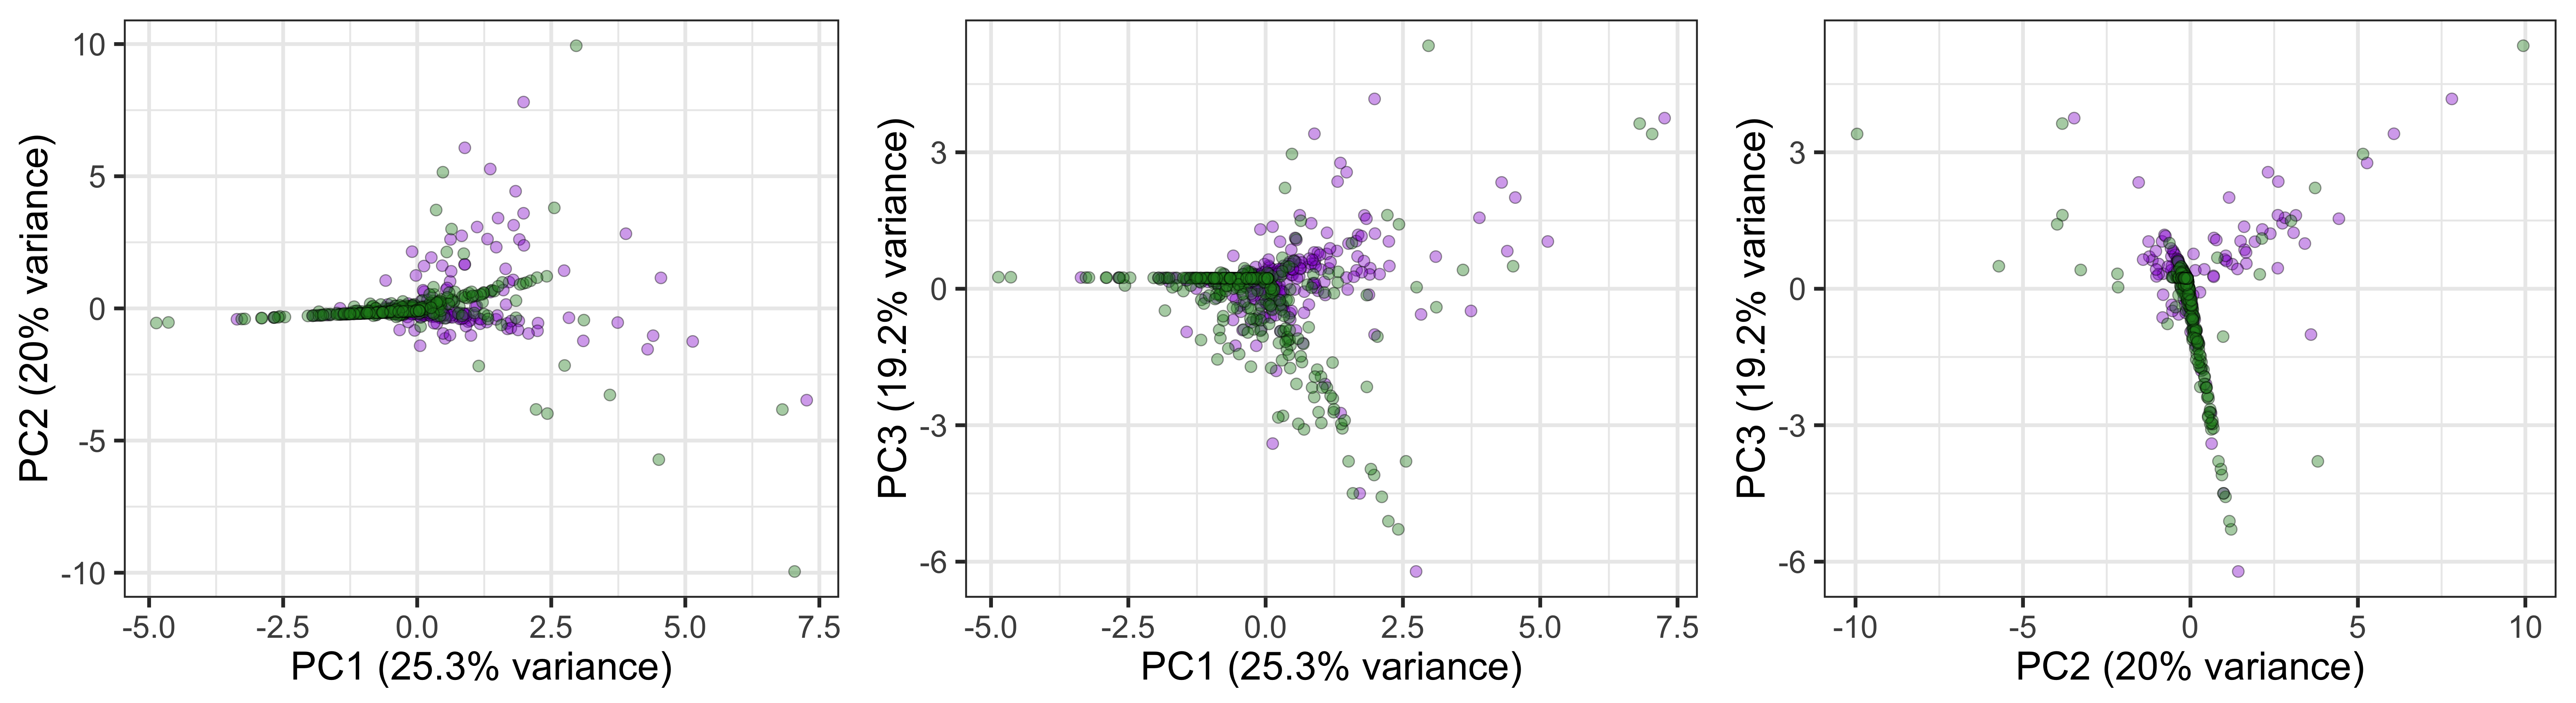
\includegraphics{pics/PCAh.png}}
    \caption{Exploratory data analysis of the \texttt{working set} using PCA for linear dimensionality reduction. Each dot in the two-dimensional space represents a gene and is coloured according to its label (green target, purple non-target)}
    \label{fig:OT_PCA}
\end{figure}

\begin{figure}[H]
\centering
    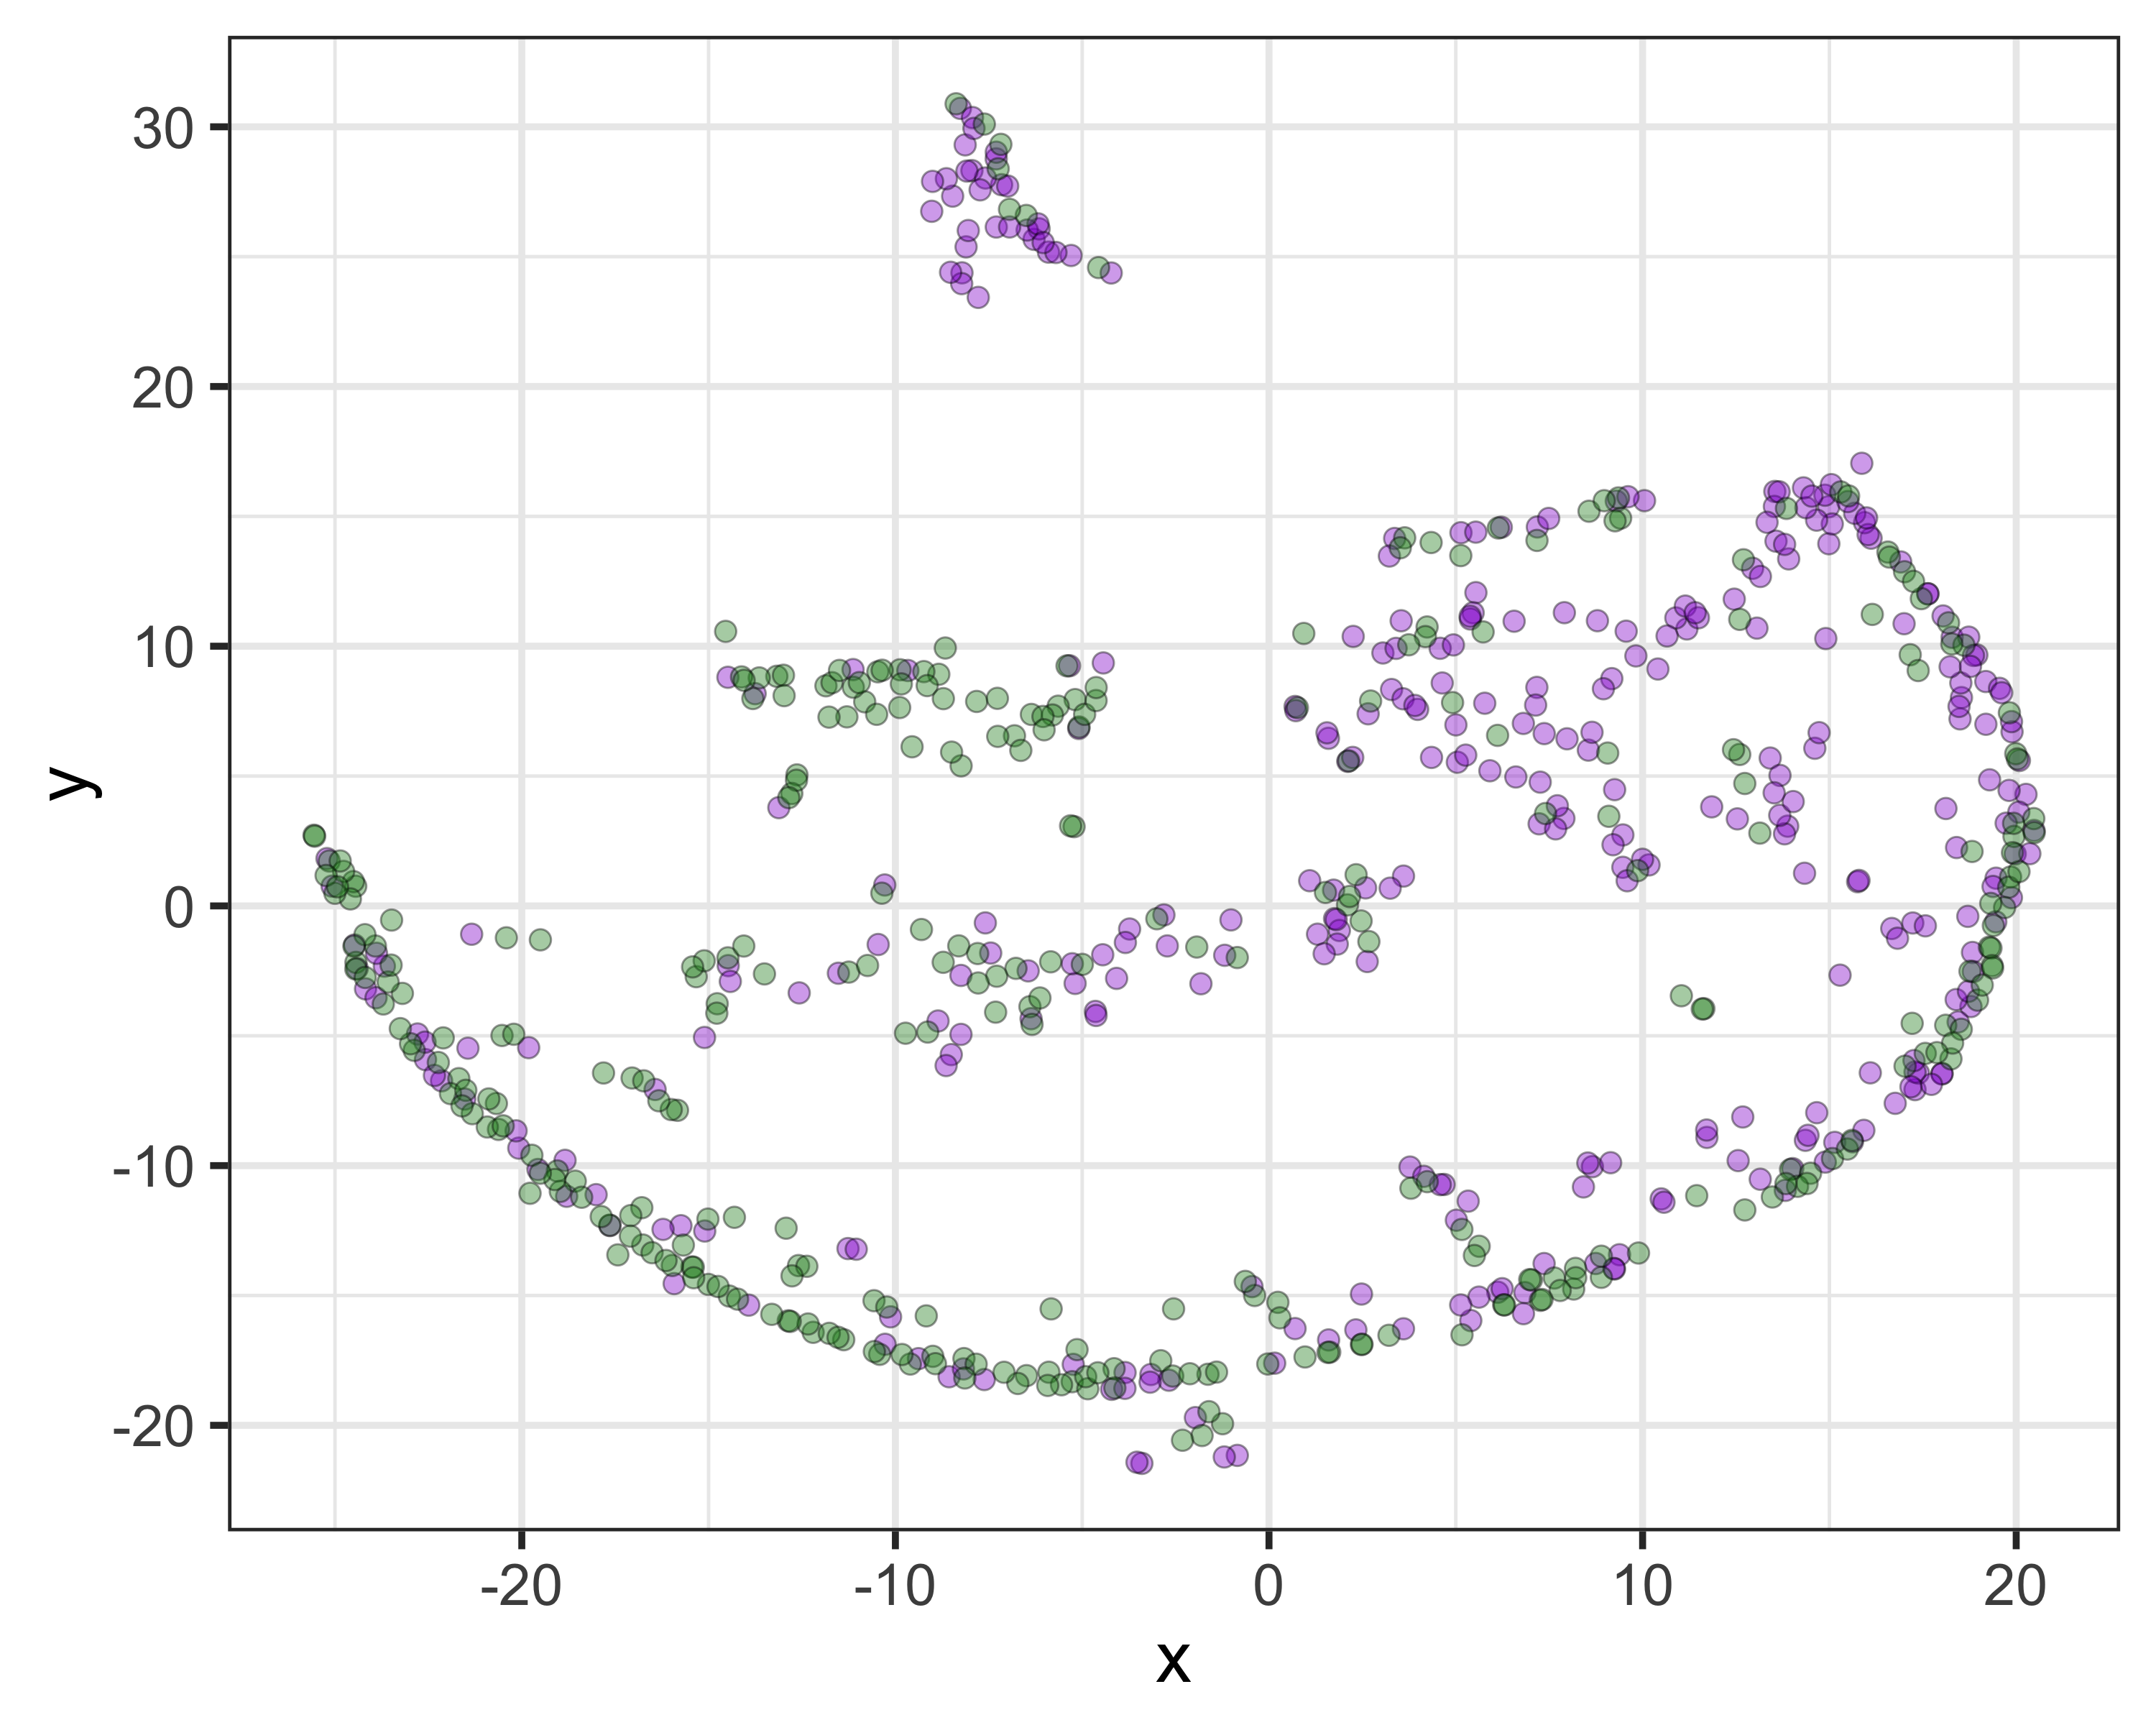
\includegraphics[width=11cm]{pics/tSNE.png}
    \caption{Exploratory data analysis of the \texttt{working set} using dimensionality reduction. The tSNE algorithm for non-linear dimensionality reduction was run a perplexity value of 30 and other default parameters. Each dot in the two-dimensional space represents a gene and is coloured according to its label (green target, purple non-target)}
    \label{fig:OT_tSNE}
\end{figure}

tSNE resulted in a rather clear separation between targets and non-targets on a two-dimensional space (see Figure \ref{fig:OT_tSNE}: most of the data points labelled as targets lie on a curved line and a gradient of targets and non-targets is present along the vertical axis. This results are clearly similar to Ferrero et al. \cite{ferrero2017}, showing that there is a distinction between therapeutic targets and non-targets in Open Targets data.

Next, they investigated the contributions of all five individual data types and their relative importance in the \texttt{working set} with two methods: (i) Chi squared test and (ii) information gaining in Figure \ref{fig:OT_features}. \texttt{animal\_model}, \texttt{rna\_expression} and \texttt{genetic\_association} showed the highest values and association with the outcome binary variable in both their and my results (see Figure \ref{fig:OT_features}).

\begin{figure}[H]
\centering
    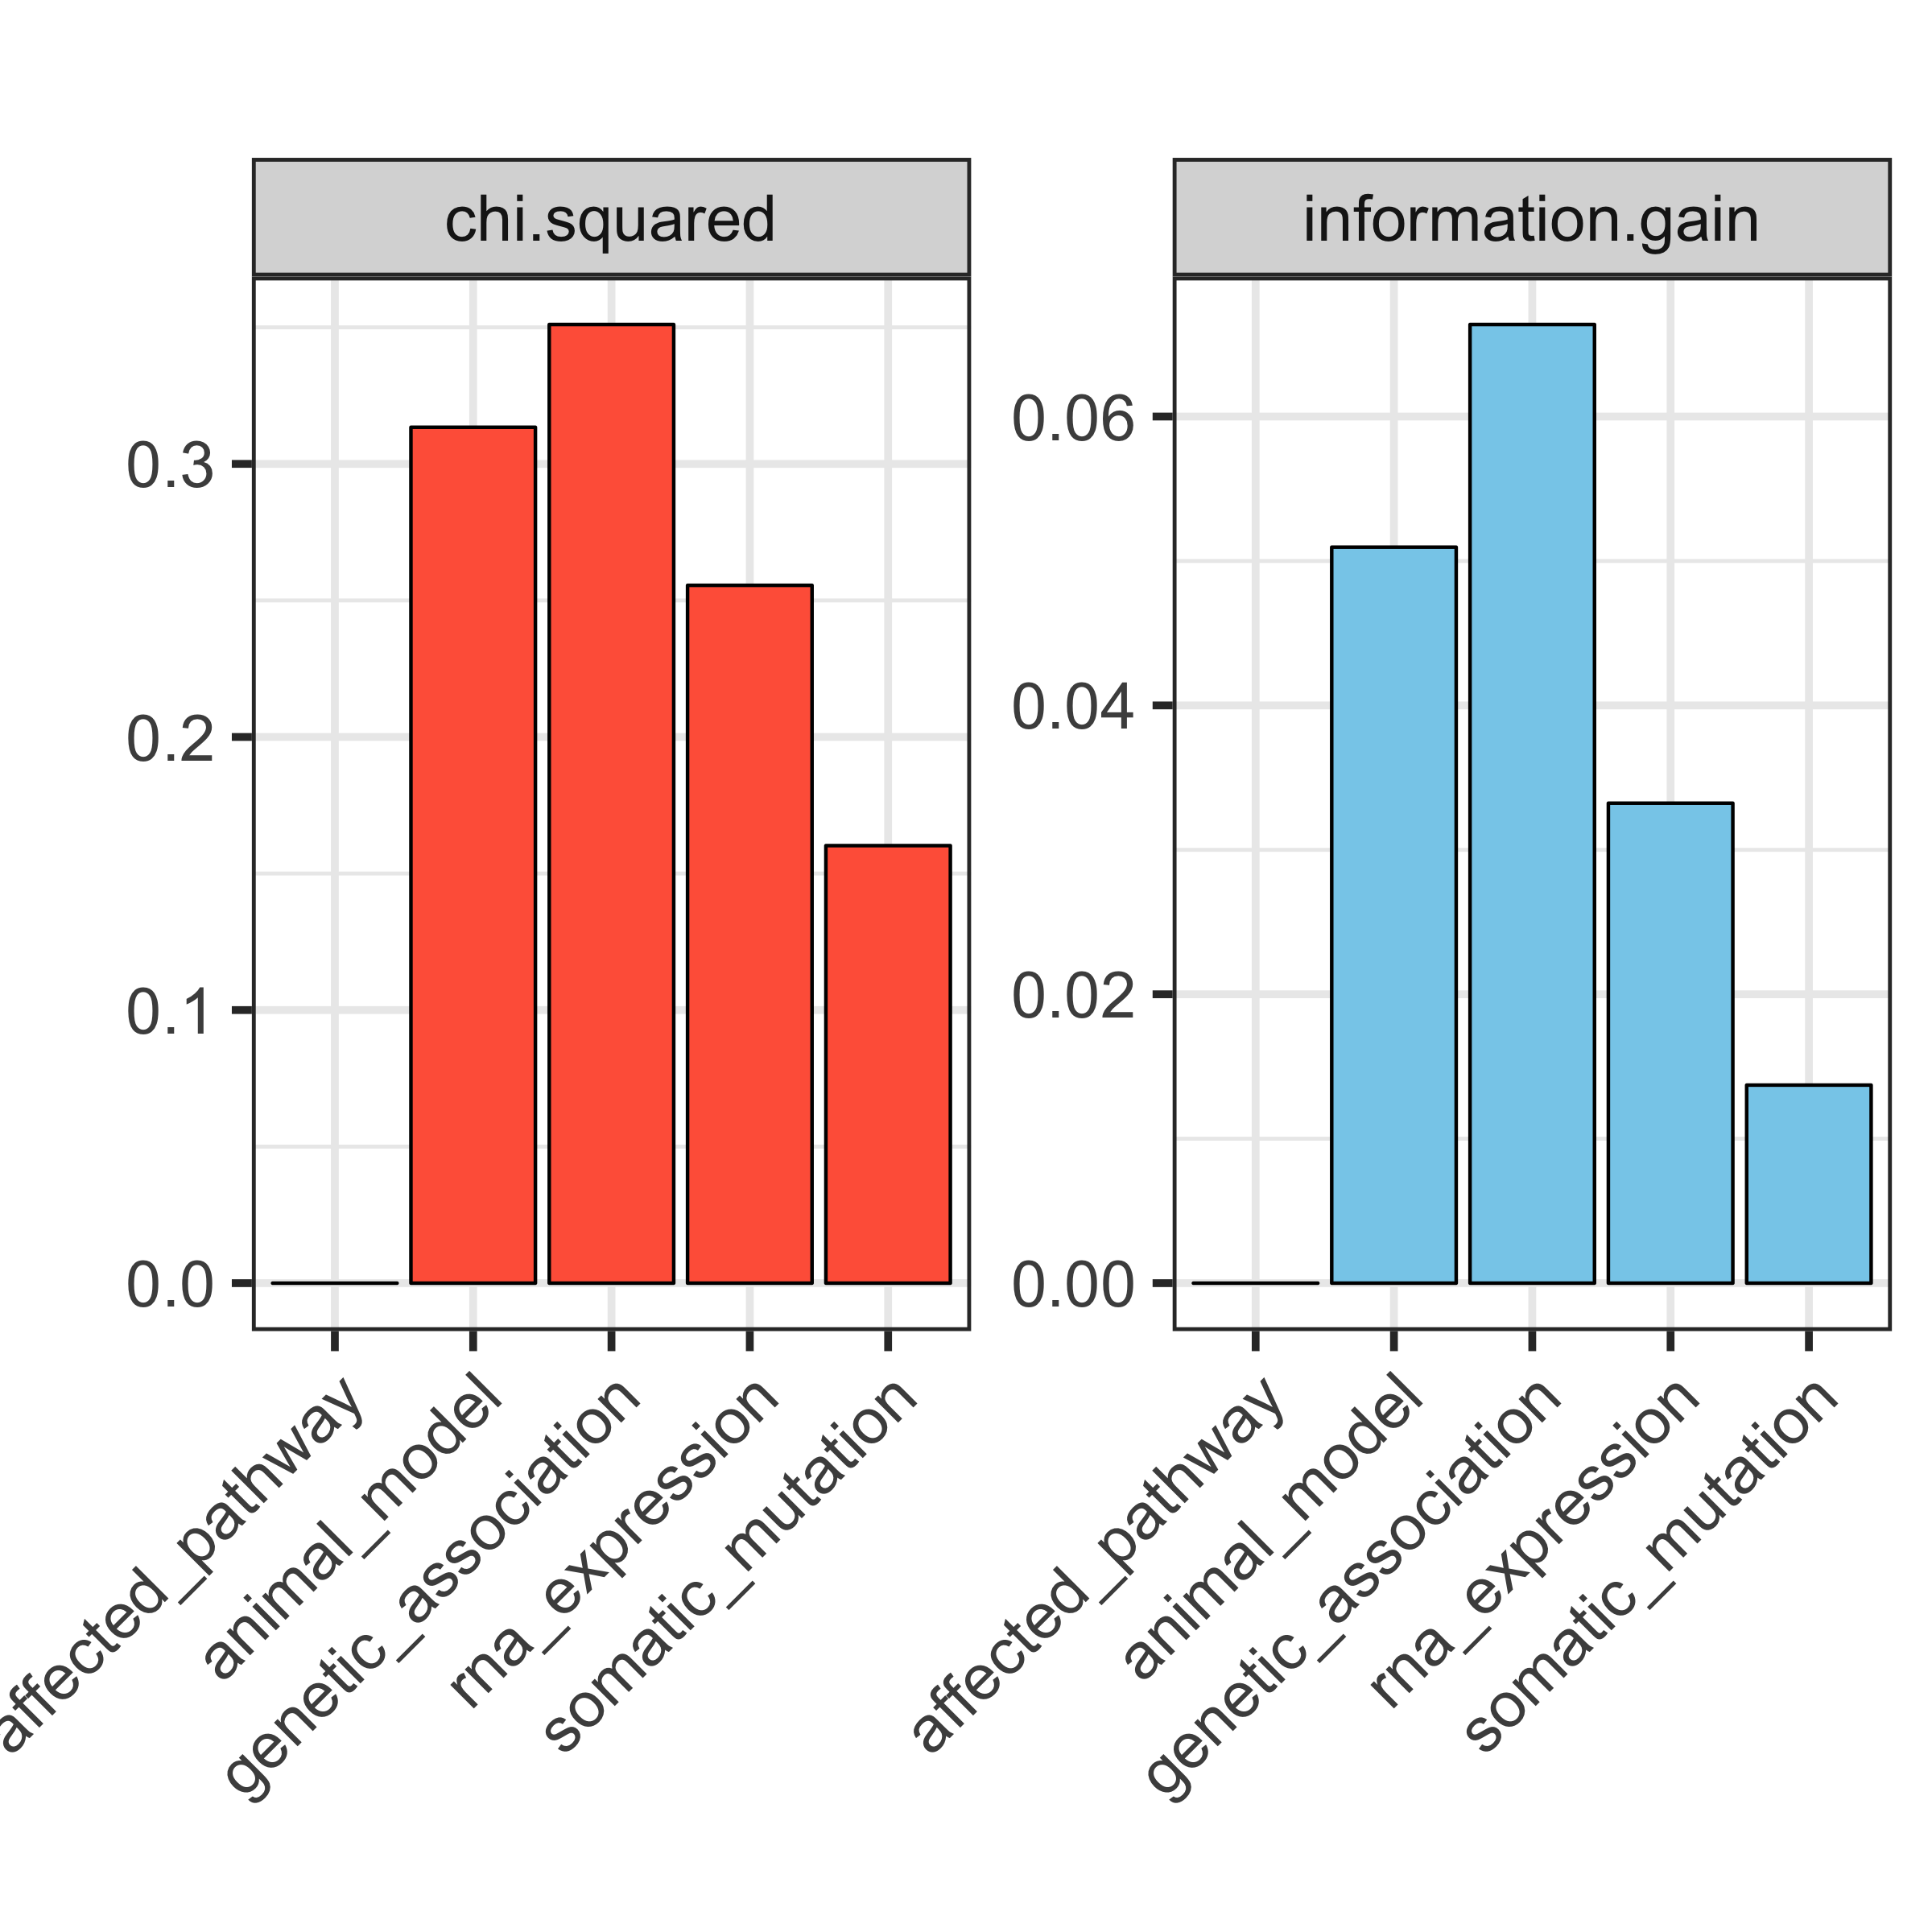
\includegraphics[width=7cm]{pics/Features.png}
    \caption{Feature importance according to two independent feature selection methods (left to right): Chi squared test and information gain with the \texttt{working set}}
    \label{fig:OT_features}
\end{figure}

They explored the classification criteria of a decision tree model to get insights into the best features for classification. Again, \texttt{animal\_model}, \texttt{rna\_expression} and \texttt{genetic\_association} were the most important features for target classification. These results are important and will be discussed in Section \ref{subsub:limitations_openTargets}.

\begin{figure}[H]
    \centering
    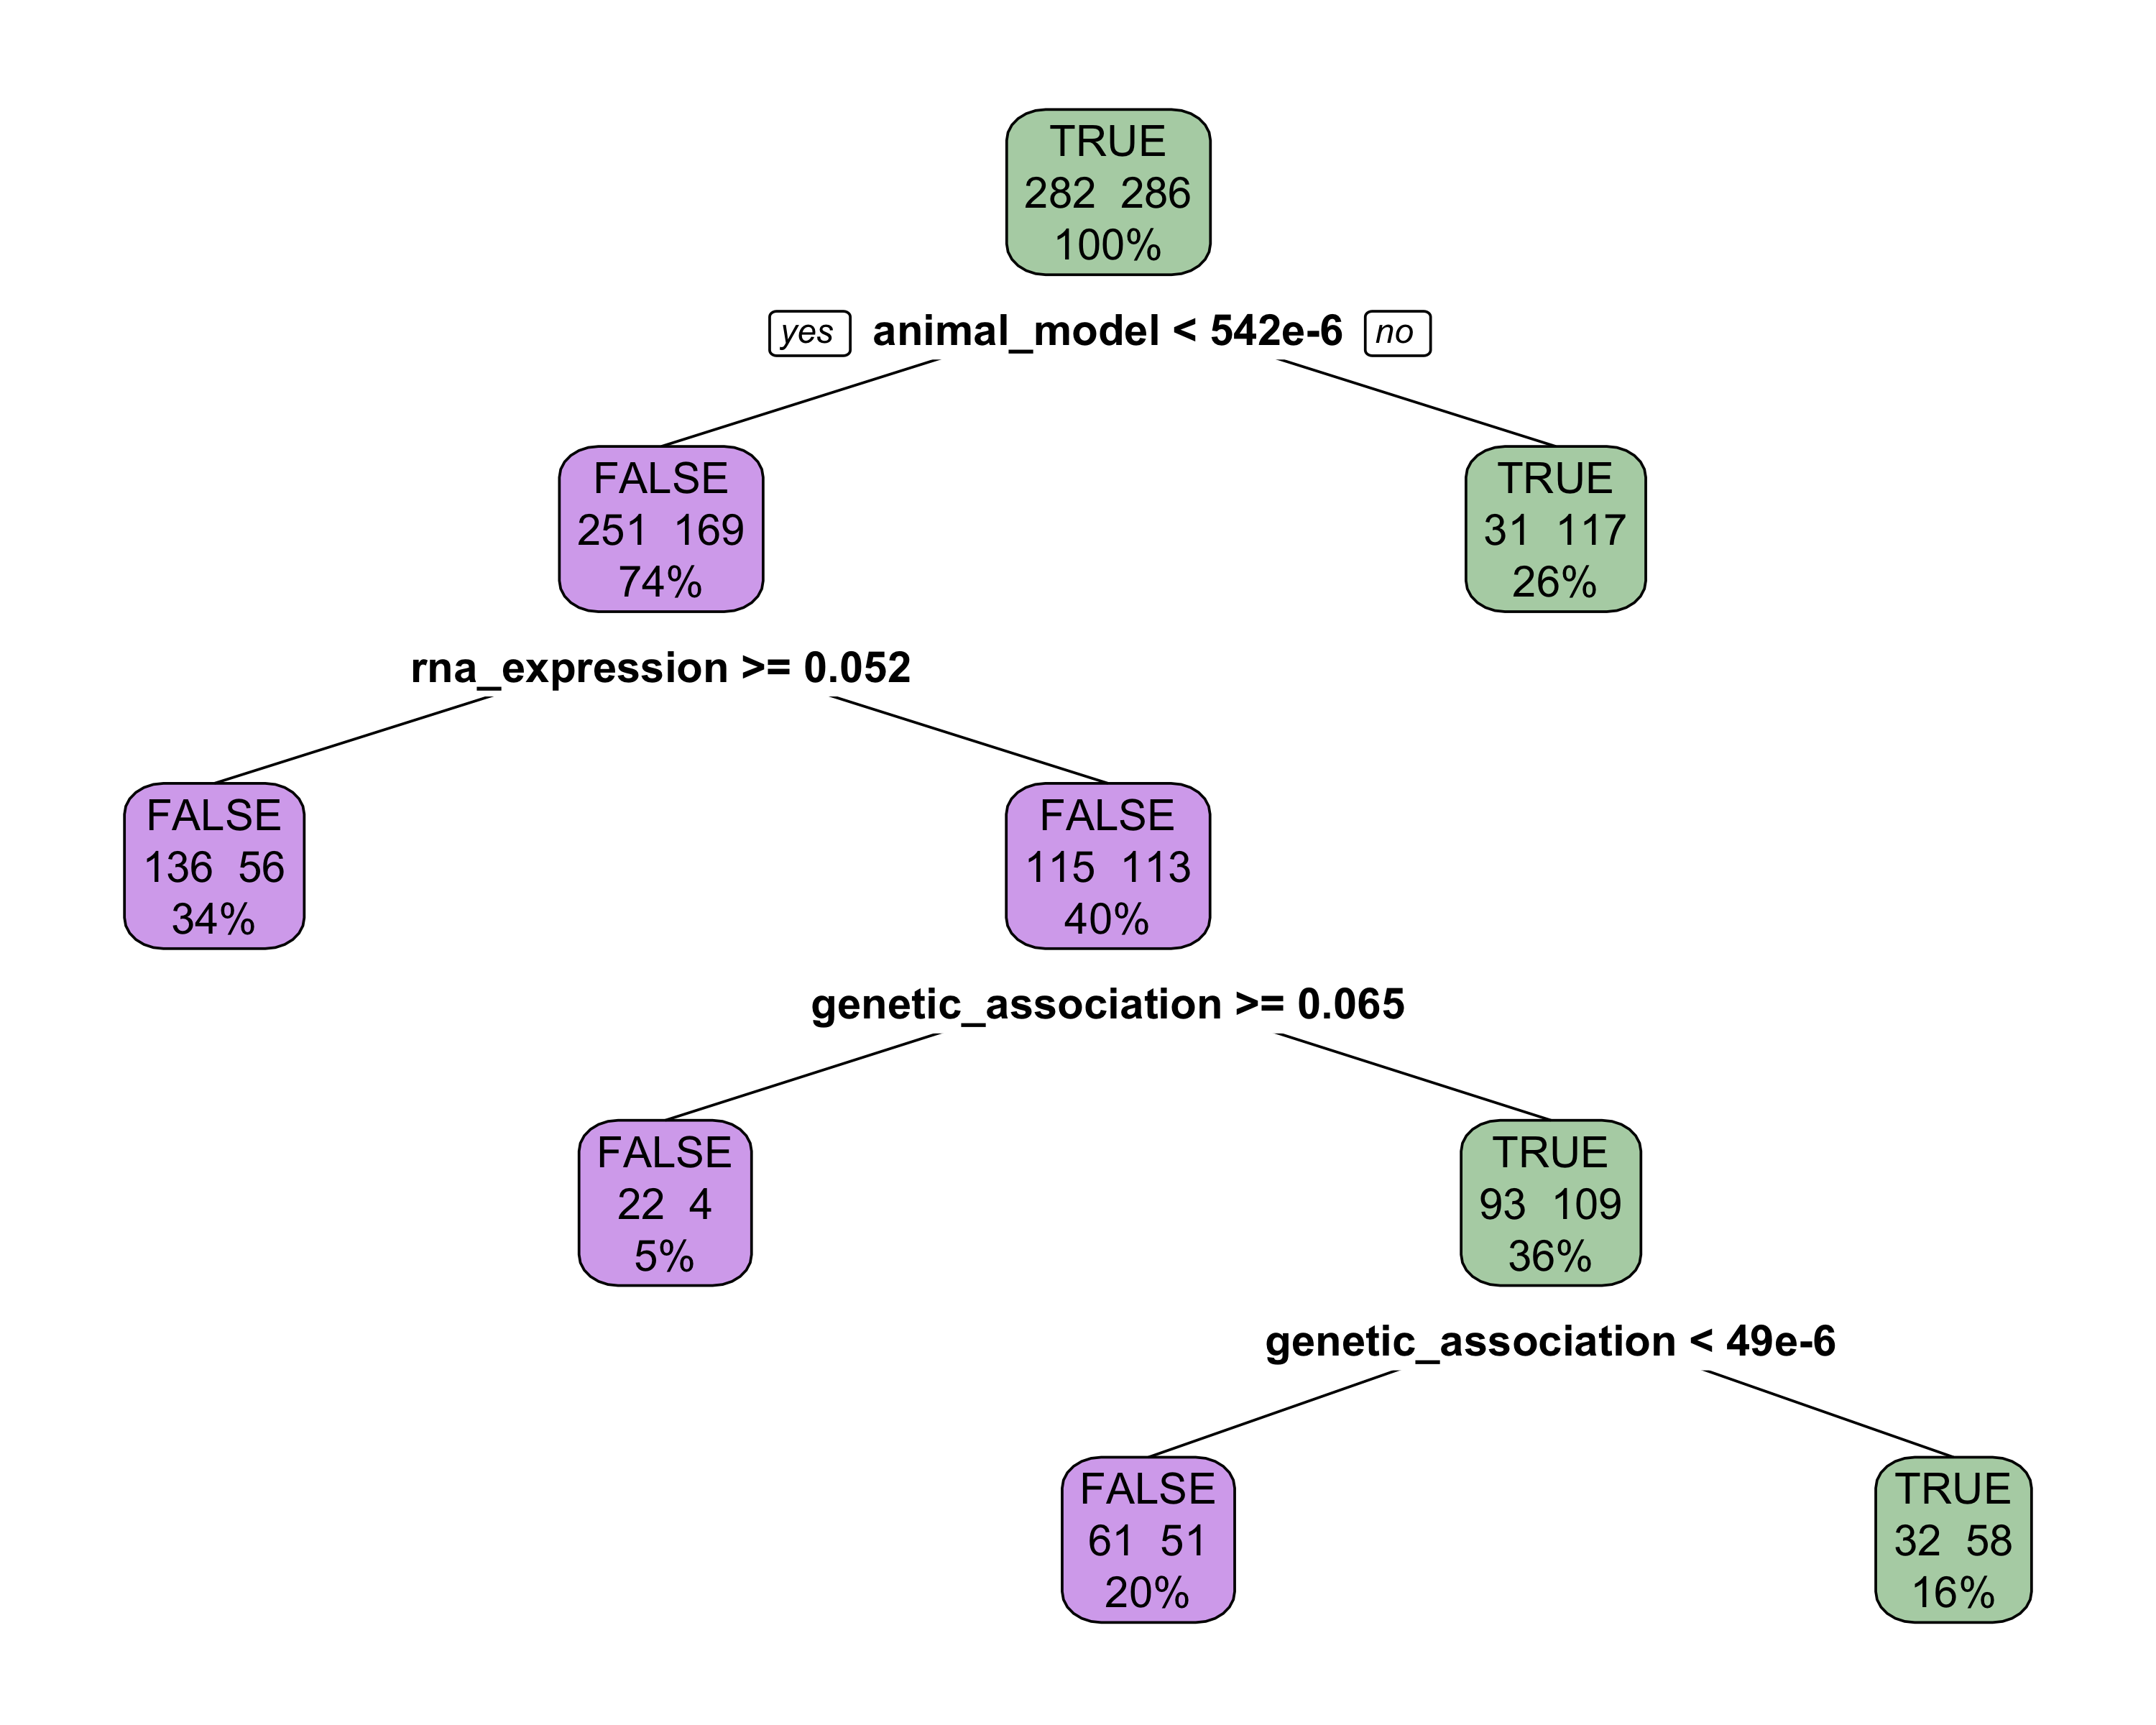
\includegraphics[width=11cm]{pics/DecisionTreeInf.png}
    \caption{Decision tree classification criteria: colours represent predicted outcome (purple non-target, green target). In each node, numbers represent (from top to bottom): outcome (FALSE: non-target, TRUE: target), number of observations in node per class (left non-target, right target), percentage of observations in node}
    \label{fig:OT_decisionTree}
\end{figure}

Open Targets used a (i) \emph{semi-supervised} approach on (ii) \emph{positive} and unlabelled data with (iii) nested cross-validation (NCV) to know if their GDAs could contain relevant information to binary classify therapeutic targets \cite{ferrero2017} according to PharmaProjects data \cite{pharmaProjects}. This aim is very important and will be discussed in \ref{subsub:limitations_openTargets}. Ferrero et al. used four different ML binary classifiers:
\begin{itemize}
    \item \textbf{Random Forest} (RF)
    \item \textbf{Support Vector Machine} (SVM) with a radial kernel
    \item Feed-forward \textbf{Neural Network} (NN) with a single hidden unit
    \item \textbf{Gradient Boosting Machine} (GBM) using the \emph{AdaBoost} exponential loss function
\end{itemize}

Why \textbf{semi-supervised}? Because the data was partially labelled. Out of the 18,104 genes, just 1,421 genes were known to be related to drugs with information about their current development phase: Preclinical, Clinical Trial, Phase I Clinical Trial, Phase II Clinical Trial, Phase III Clinical Trial, Pre-registration, Registered, Launched, (Failed, or Abandoned? this will be negative labelling) according to Informa Pharmaprojects data \cite{pharmaProjects}. Restrictions apply to the availability of the Pharmaprojects data, which was used under license for the current study, and so is not publicly available \cite{ferrero2017}. Failed or abandoned projects according to Pharmaprojects were ignored \cite{ferrero2017}. It is uncertain whether the remaining 16,683 genes may become a potential target in the future \cite{ferrero2017}. Semi-supervised methods tackle problems where there is a mixture of labelled and unlabelled data.
    
Why \textbf{positive} labelled? Because all genes known to be related to drugs are the ones that are in any of the above categories, labelled as belonging to an active or \emph{positive} drug discovery process. This type of problem is known as Positive-Unlabelled or PU learning. To account for this problem, bootstrap aggregating (\emph{bagging}) with 100 iterations was applied to the SVM, the NN and the GBM classifiers. RF does \emph{bagging} by default in R 3.3.0
    
Why \textbf{nested cross-validation} (NCV)? Because NCV generalises the estimation error of the model and its hyperparameters in an inner loop. Non-NCV biases the model yielding an overly optimistic score. A comparison between NCV and non-NCV in Python can be found \href{https://goo.gl/soHYT7}{elsewhere}. Ferrero et al. used NCV with a 4-fold inner loop to optimise the hyperparameters and a 4-fold outer loop to estimate the performance in the \texttt{training set}. \emph{Hyperparameters} are parameters that are intrinsic to the defined model and are set prior to the training process. The \emph{parameters} of the model are derived from the ML training process. With NCV there is a inner loop to search for the best hyperparameters and, secondly, an outer loop to optimise the parameters.


Different measures were used to assess the classifiers (RF, SVM, NN and GBM):
\begin{itemize}
    \item Receiver operating characteristic (ROC) curves in Figure \ref{fig:OT_ROC}
    \item Precision-recall curves in Figure \ref{fig:OT_precisionRecall}
    \item Misclassification errors in Figure \ref{fig:OT_MmceBoxplots}
    \item Box plots for the distribution of the following measures: area under the curve (AUC), accuracy, F1 measure, precision, recall/sensitivity ratio, and specificity in Figure \ref{fig:OT_OtherPlots}
\end{itemize}

\begin{figure}[H]
    \centering
    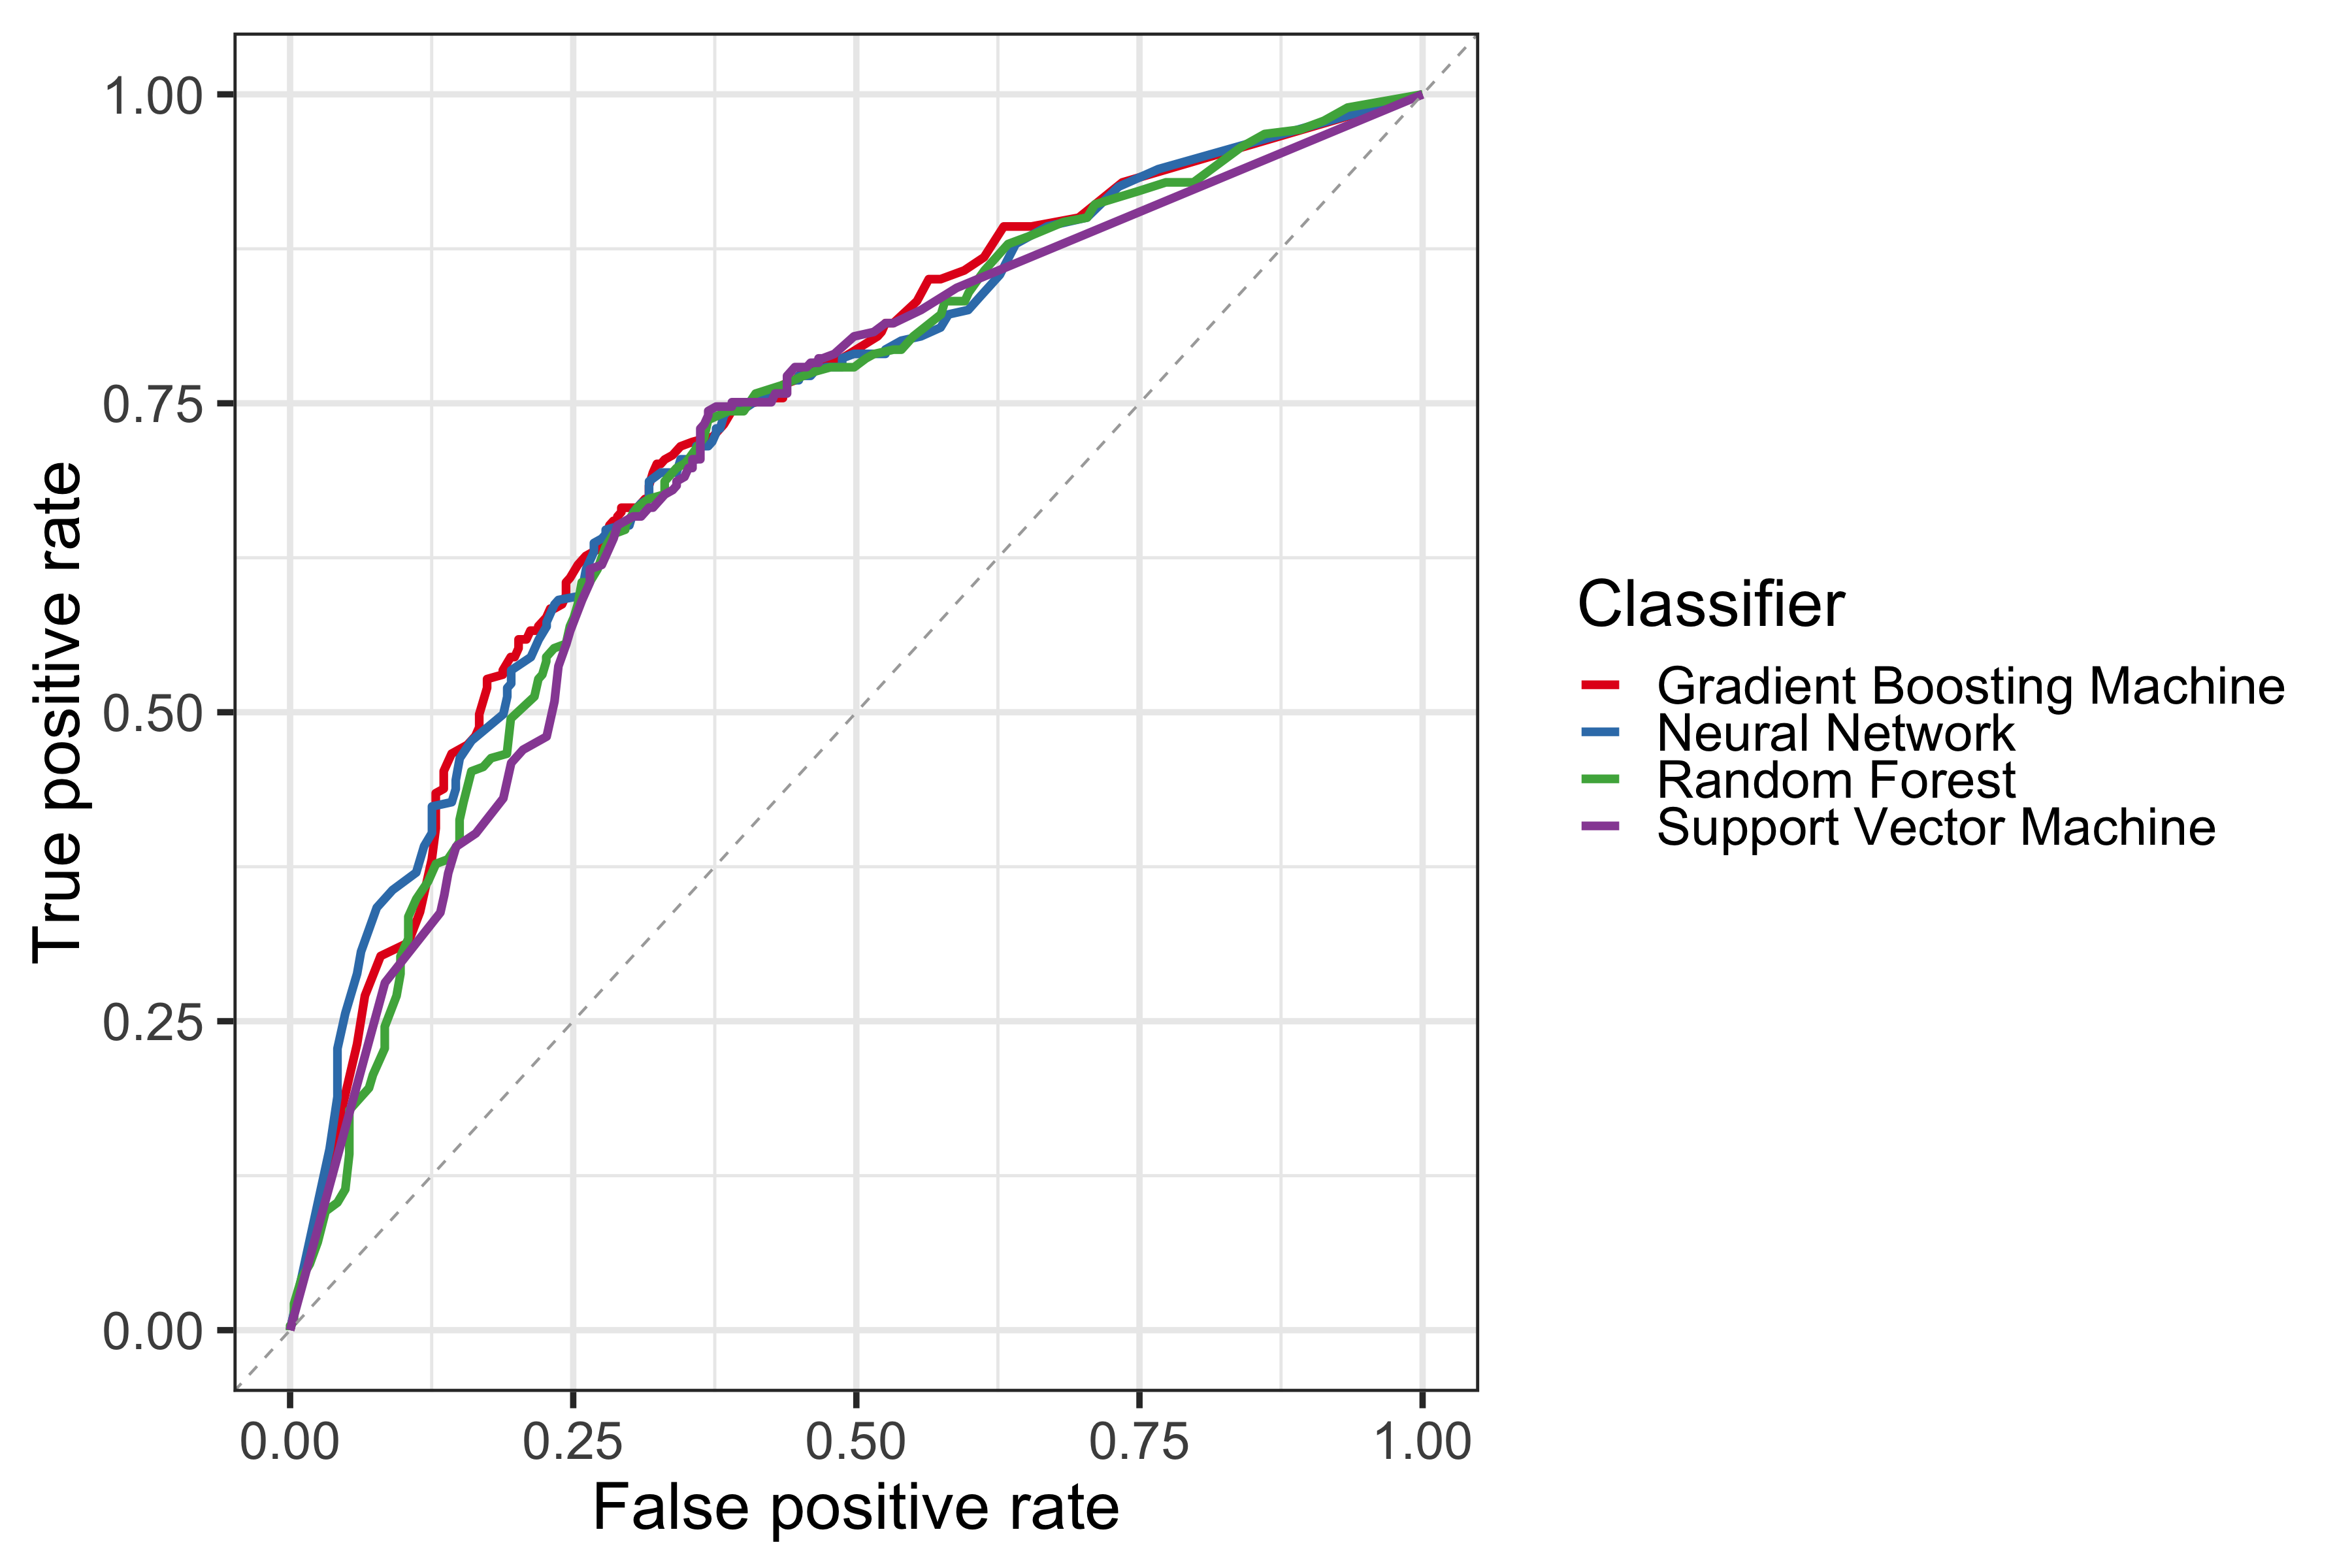
\includegraphics[width=11cm]{pics/BenchmarkROC.png}
    \caption{Estimated receiver operating characteristic (ROC) curve of trained classifiers as assessed by nested cross-validation on the training set \label{fig:OT_ROC}}
\end{figure}

\begin{figure}[H]
    \centering
    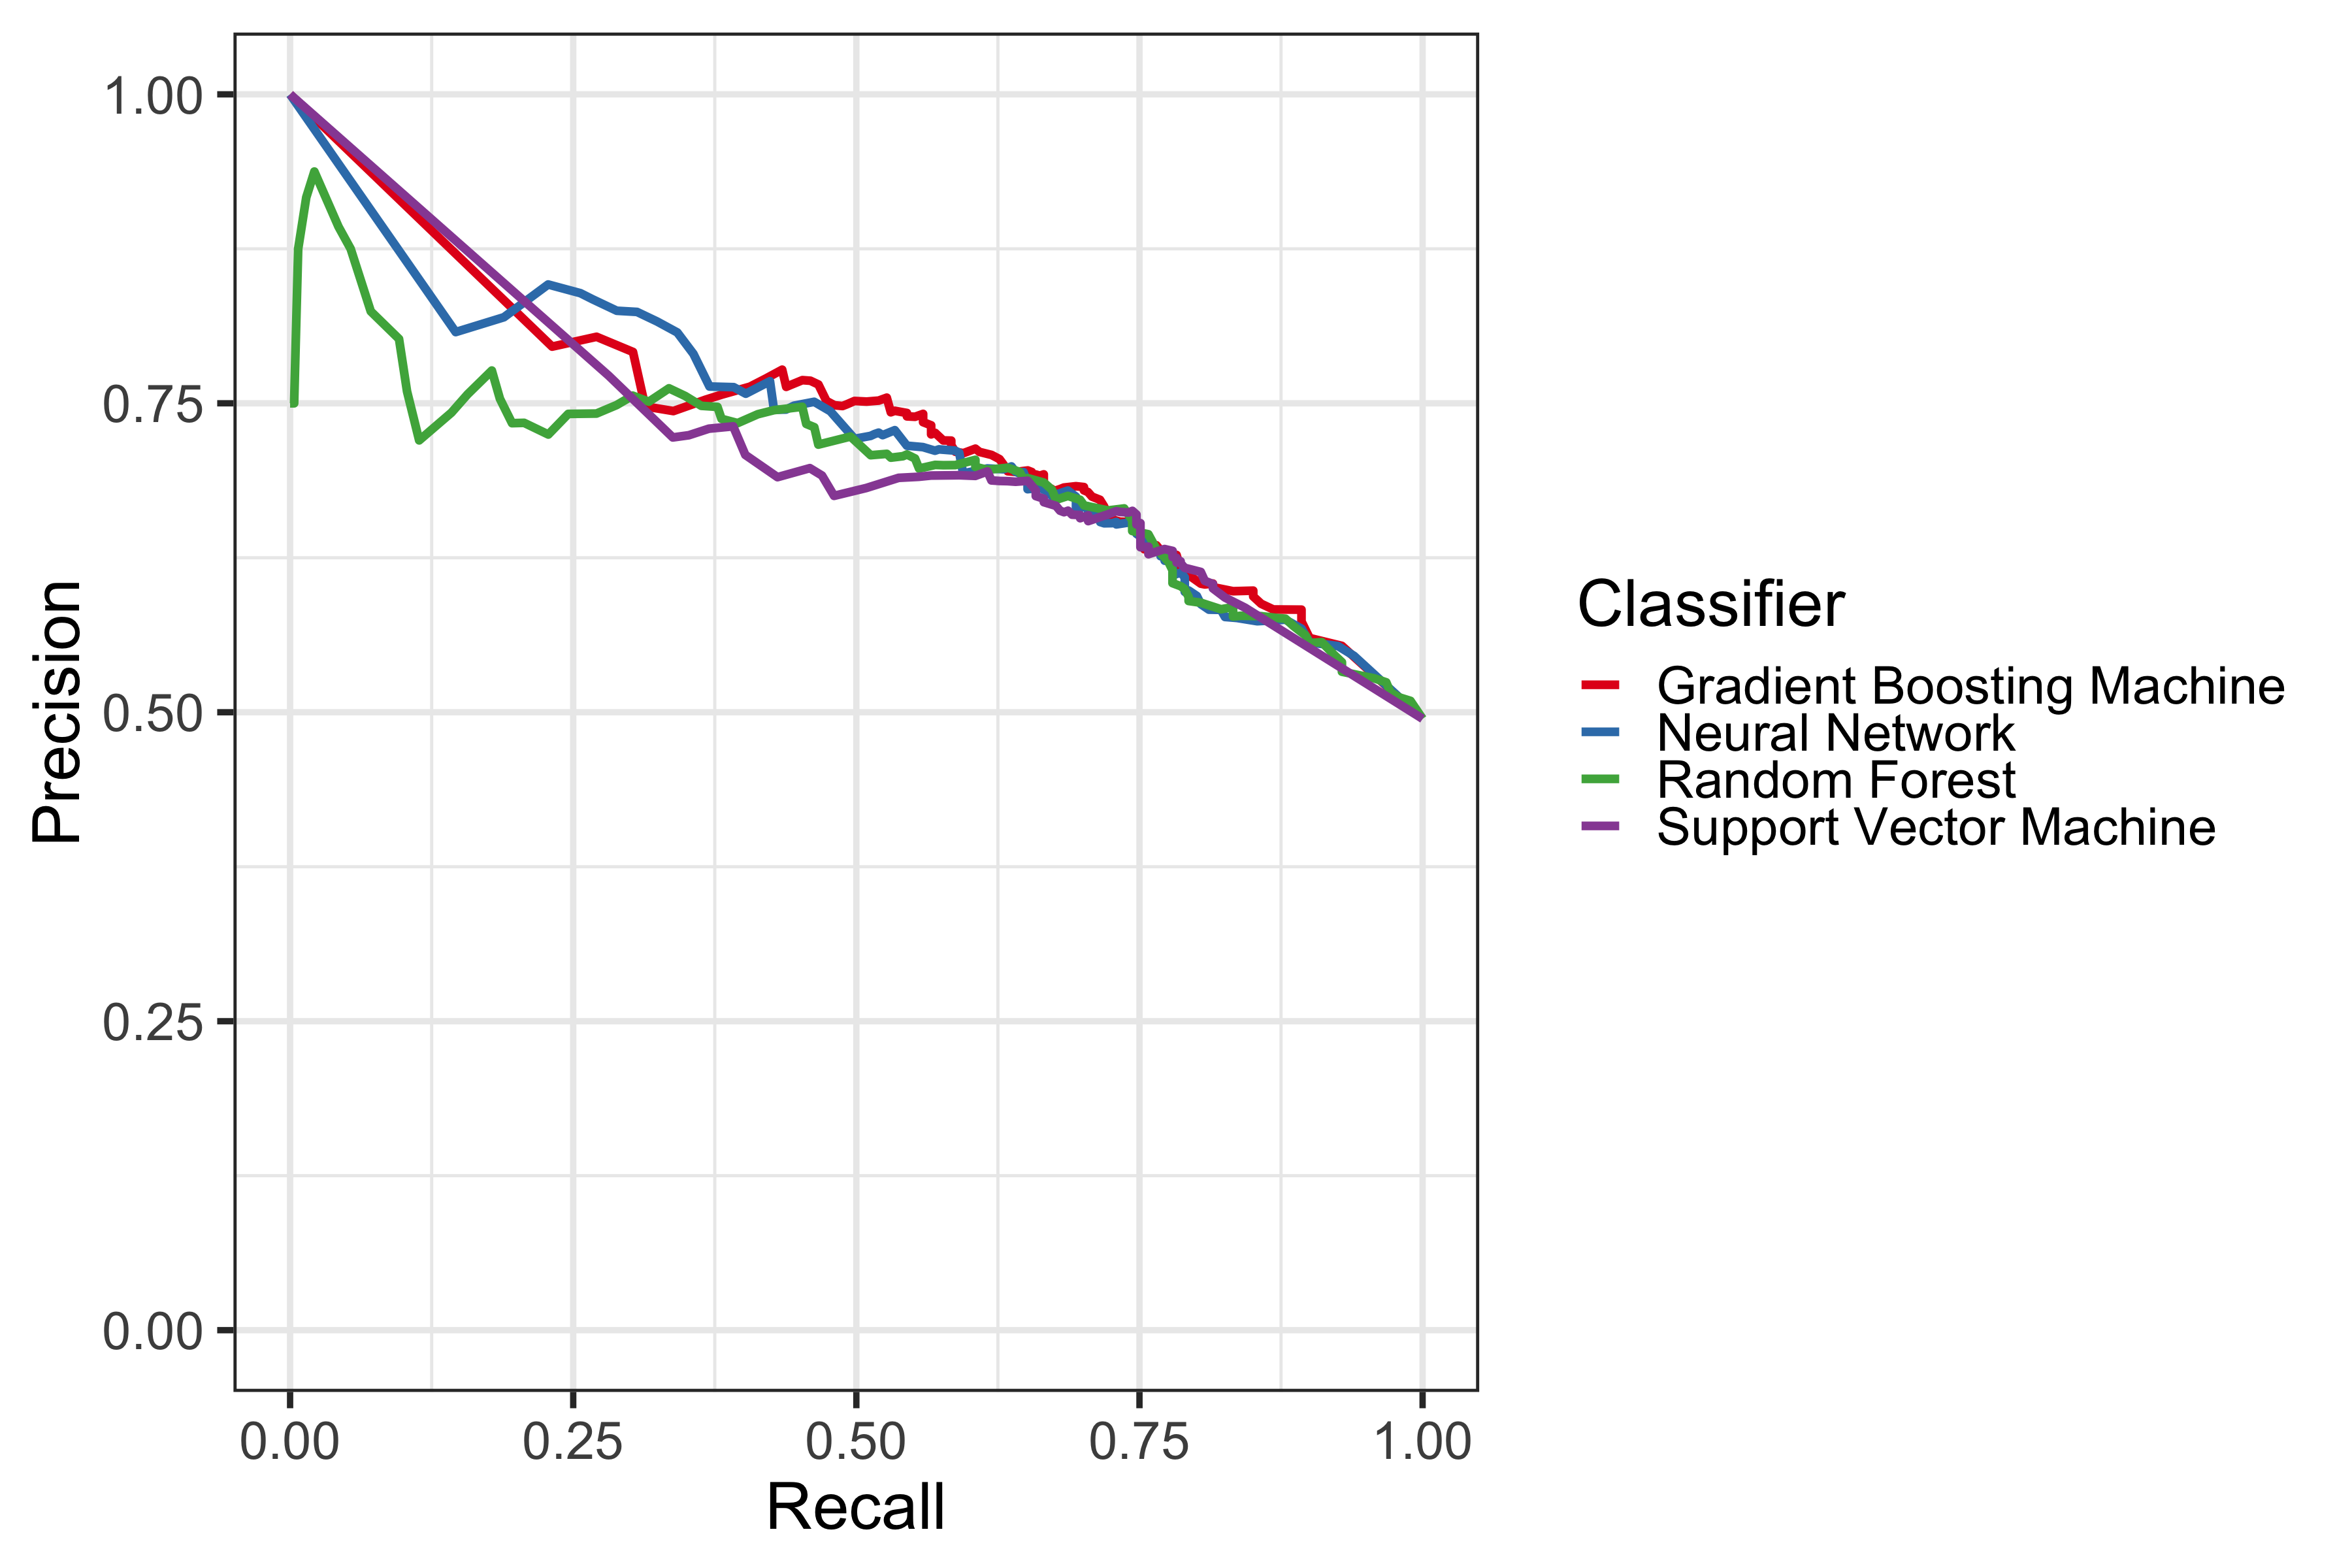
\includegraphics[width = 11cm]{pics/BenchmarkPR.png}
    \caption{Precision-–recall curves of the four trained classifiers as assessed by NCV on the \texttt{training set} \label{fig:OT_precisionRecall}}
\end{figure}

\begin{figure}[H]
    \centering
    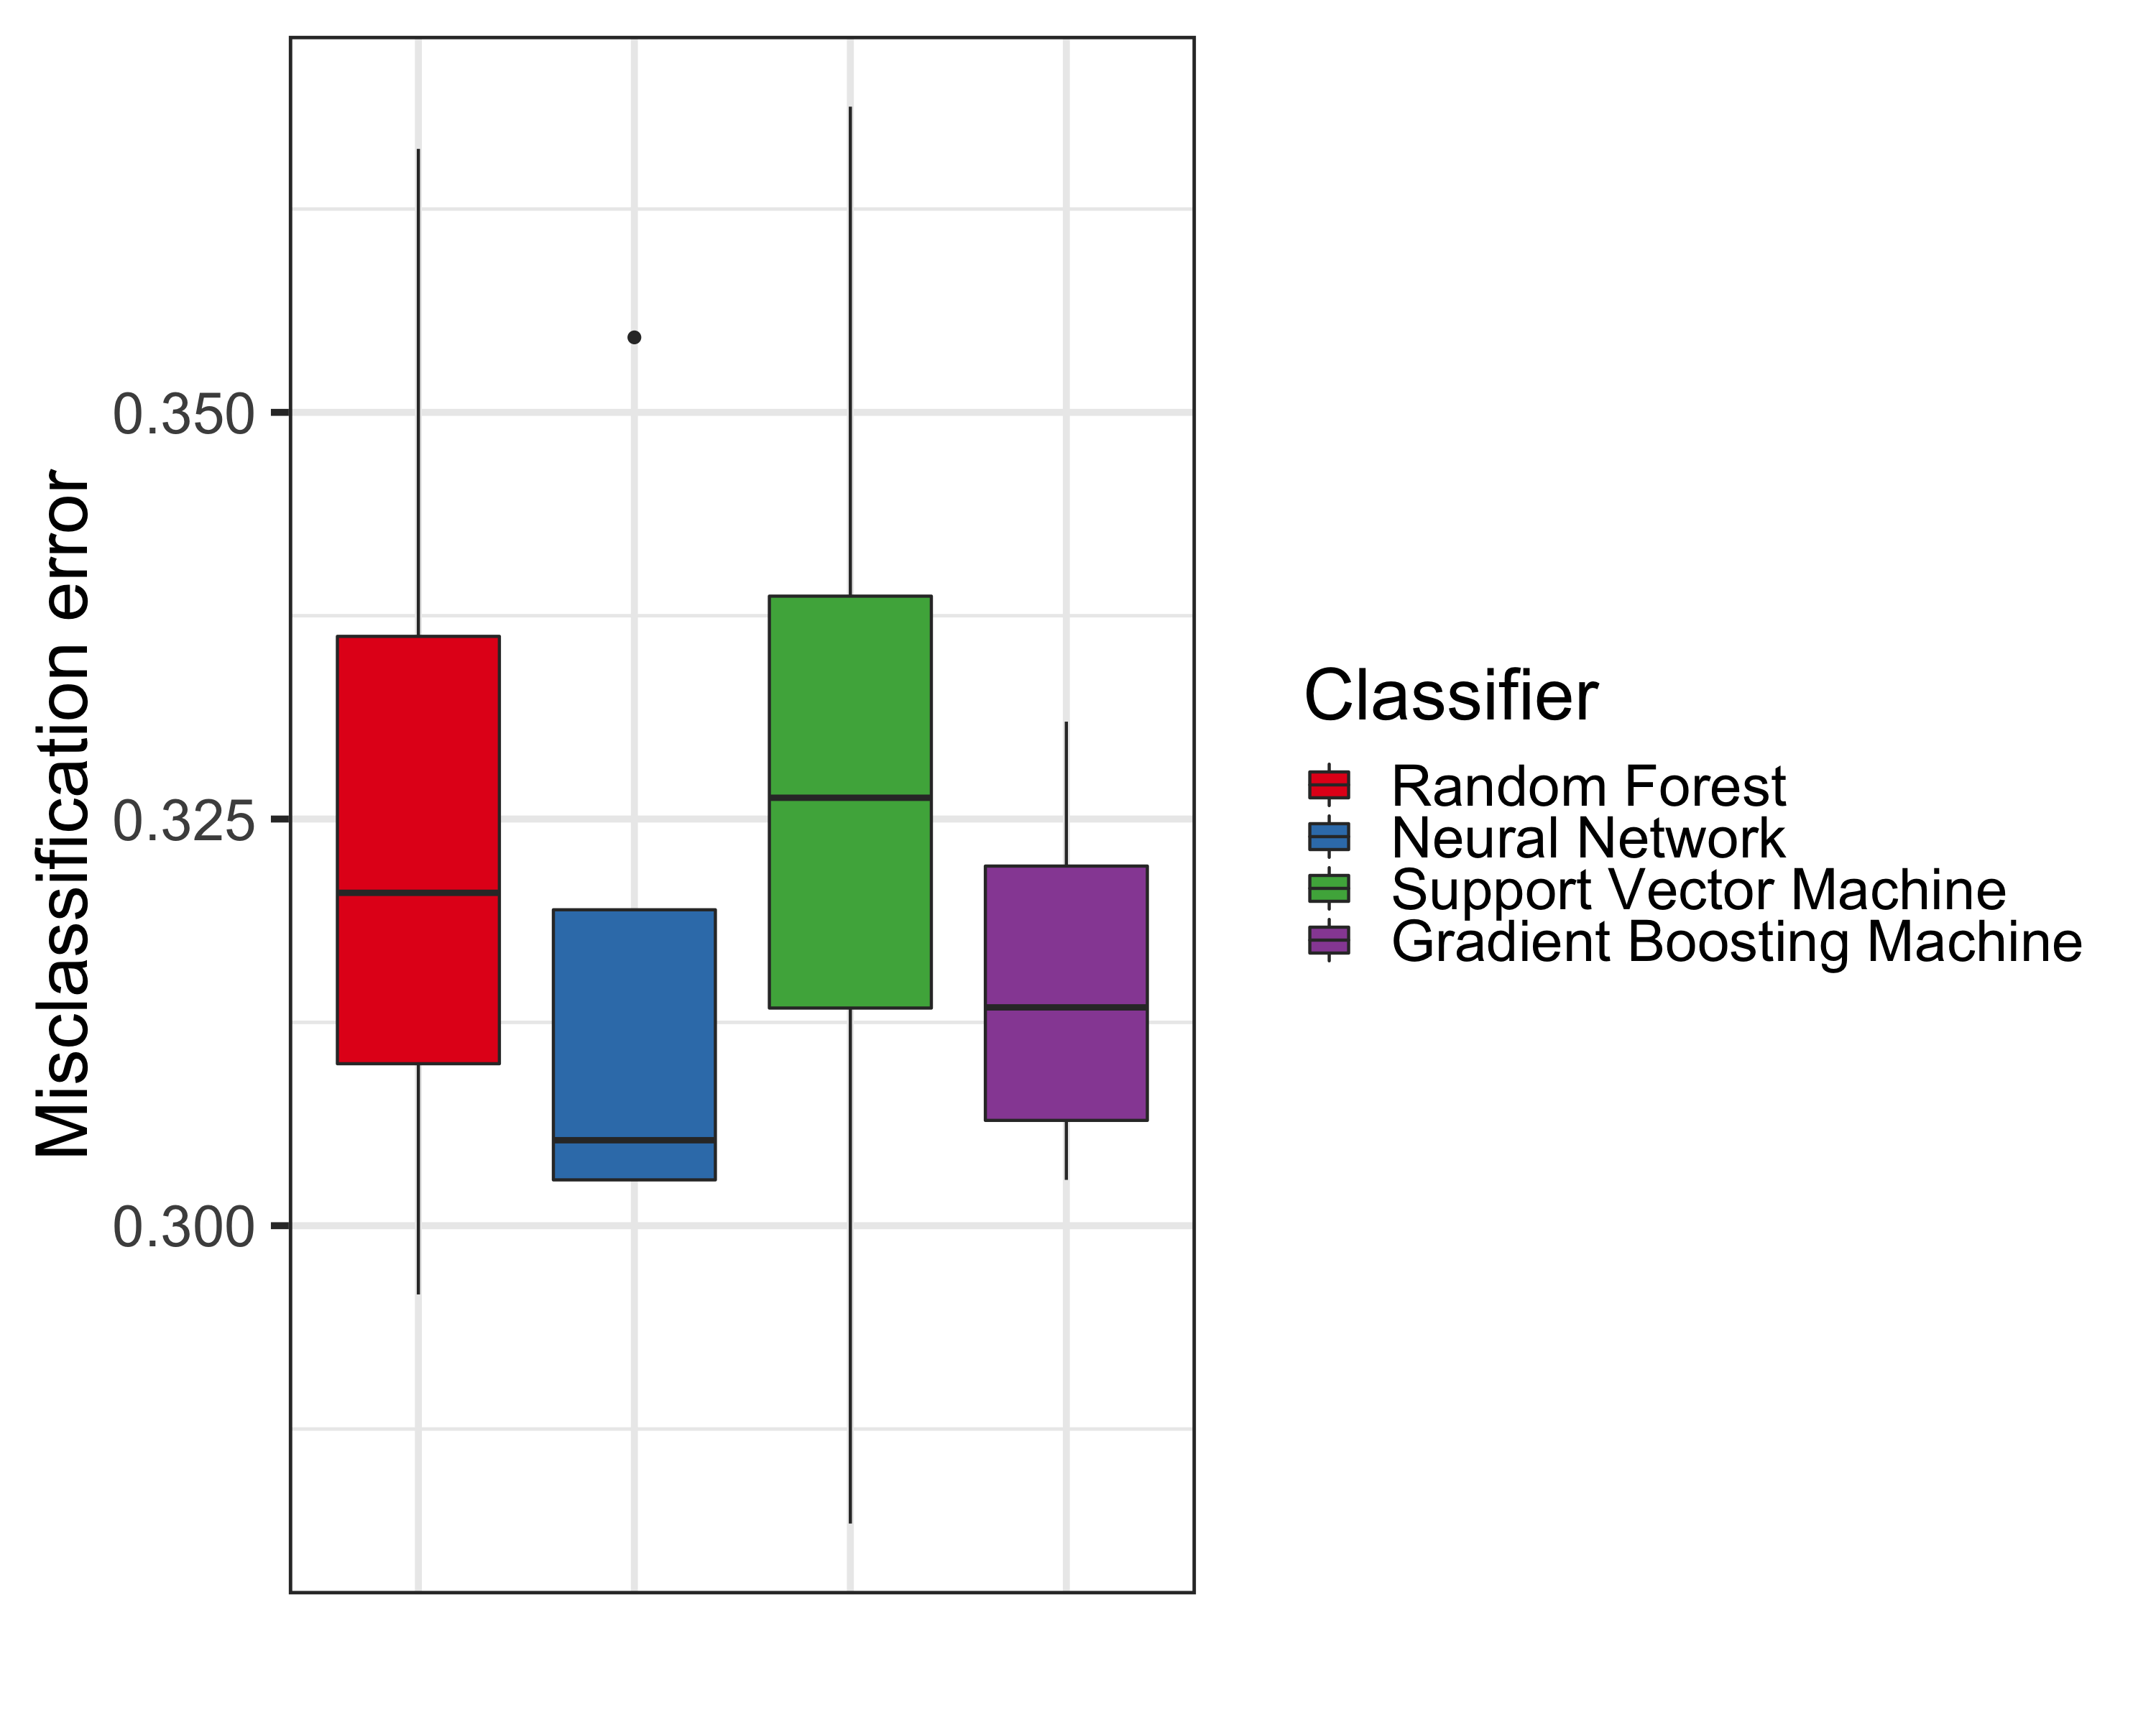
\includegraphics[width = 9cm]{pics/BenchmarkMmceBoxplots.png}
    \caption{Box plot showing the distribution of misclassification errors for the four trained classifiers, as assessed by NCV on the \texttt{training set} \label{fig:OT_MmceBoxplots}}
\end{figure}

\begin{figure}[H]
    \centering
    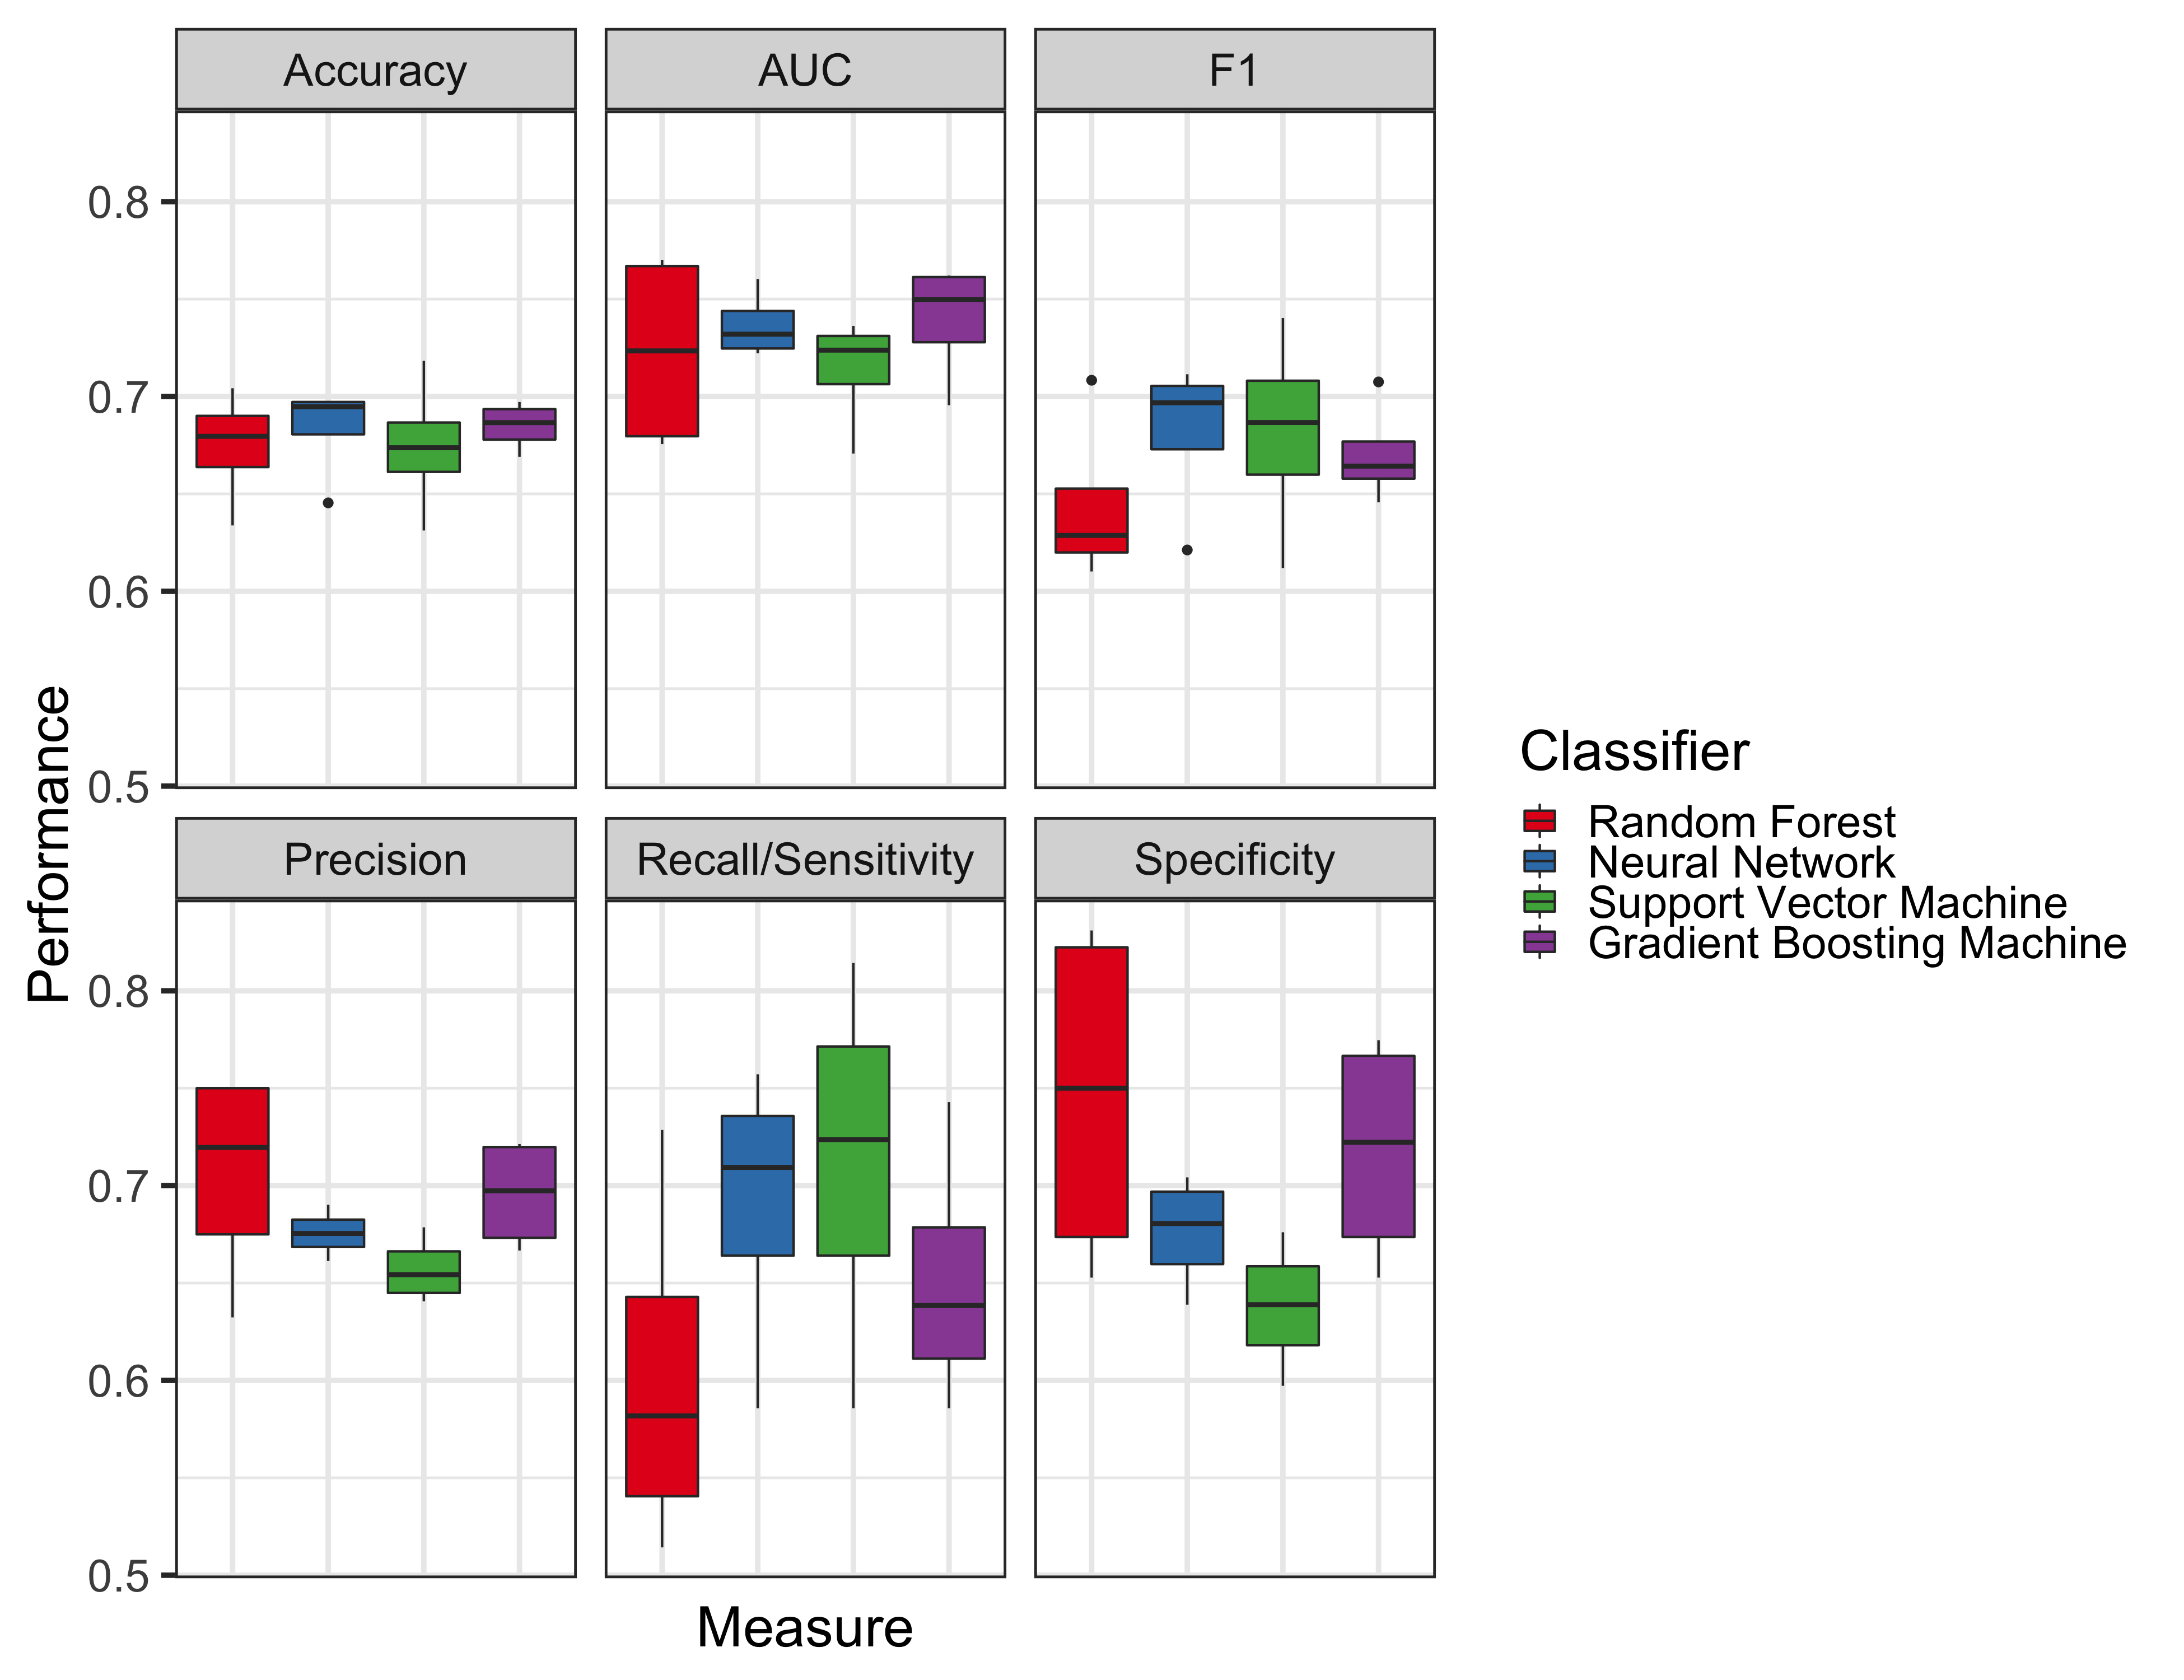
\includegraphics[width = 13cm]{pics/BenchmarkOtherBoxplots.png}
    \caption{Box plots showing distributions of the following measures for the four trained classifiers: accuracy, AUC, F1 measure, precision, recall/sensitivity and specificity, as assessed by NCV on the \texttt{training set} \label{fig:OT_OtherPlots}}
\end{figure}

Overall, all algorithms had comparable accuracy, AUC, and precision (see Figure \ref{fig:OT_OtherPlots}). These results are slightly lower than the ones reported by Ferrero et al. \cite{ferrero2017} (See my results in Table \ref{tab:David_perf_train_mean} and Ferrero's results in Table \ref{tab:OT_perf_train_mean}). 

\begin{table}[H]
\centering
\begin{tabular}{c|c|c|c|c|c|c|c}
Classifier & MMCE  & Accuracy   & AUC   & Recall/Sensitivity   & Specificity   & Precision   & F1    \\
\hline
RF & 0.326 & 0.674 & 0.723 & 0.602 & 0.746 & 0.705 & 0.644 \\
NN & 0.317 & 0.683 & 0.737 & 0.690 & 0.676 & 0.676 & 0.682 \\
SVM & 0.326 & 0.674 & 0.714 & 0.712 & 0.638 & 0.657 & 0.681 \\
GBM & 0.315 & 0.685 & 0.739 & 0.651 & 0.718 & 0.696 & 0.670
\end{tabular}
\caption{\textbf{David results}. Mean \texttt{training set} performance measures (mean misclassification error, mean accuracy, mean AUC, mean recall/sensitivity ratio, mean specificity, mean precision, mean F1 measure) for all classifiers estimated by NCV \label{tab:David_perf_train_mean}}
\end{table}

\begin{table}[H]
\centering
\begin{tabular}{c|c|c|c|c|c|c|c}
Classifier & MMCE  & Accuracy   & AUC   & Recall/Sensitivity   & Specificity   & Precision   & F1    \\
\hline
RF         & 0.302 & 0.698 & 0.761 & 0.596 & 0.802 & 0.753 & 0.665 \\
NN         & 0.303 & 0.697 & 0.758 & 0.610 & 0.785 & 0.742 & 0.670 \\
SVM        & 0.317 & 0.683 & 0.733 & 0.592 & 0.775 & 0.729 & 0.652 \\
GBM        & 0.297 & 0.703 & 0.752 & 0.637 & 0.771 & 0.738 & 0.683
\end{tabular}
\caption{\textbf{Open Targets \cite{ferrero2017}}. Mean \texttt{training set} performance measures (mean misclassification error, mean accuracy, mean AUC, mean recall/sensitivity ratio, mean specificity, mean precision, mean F1 measure) for all classifiers estimated by NCV \label{tab:OT_perf_train_mean}}
\end{table}

Finally, Ferrero et al. explored how consistent was the target predictions across all four trained binary classifiers in the \texttt{training set}. All four algorithms agreed on the classification of the majority of the observations in the \texttt{training set} for both targets (47.74\% in my results versus 66.4\% in Ferrero et al.) and non-targets (55.55\% in my results versus 75.2\% in Ferrero et al.). Venn diagrams are in Figure \ref{fig:OT_venn}.

\begin{figure}[H]
\resizebox{\textwidth}{!}{
    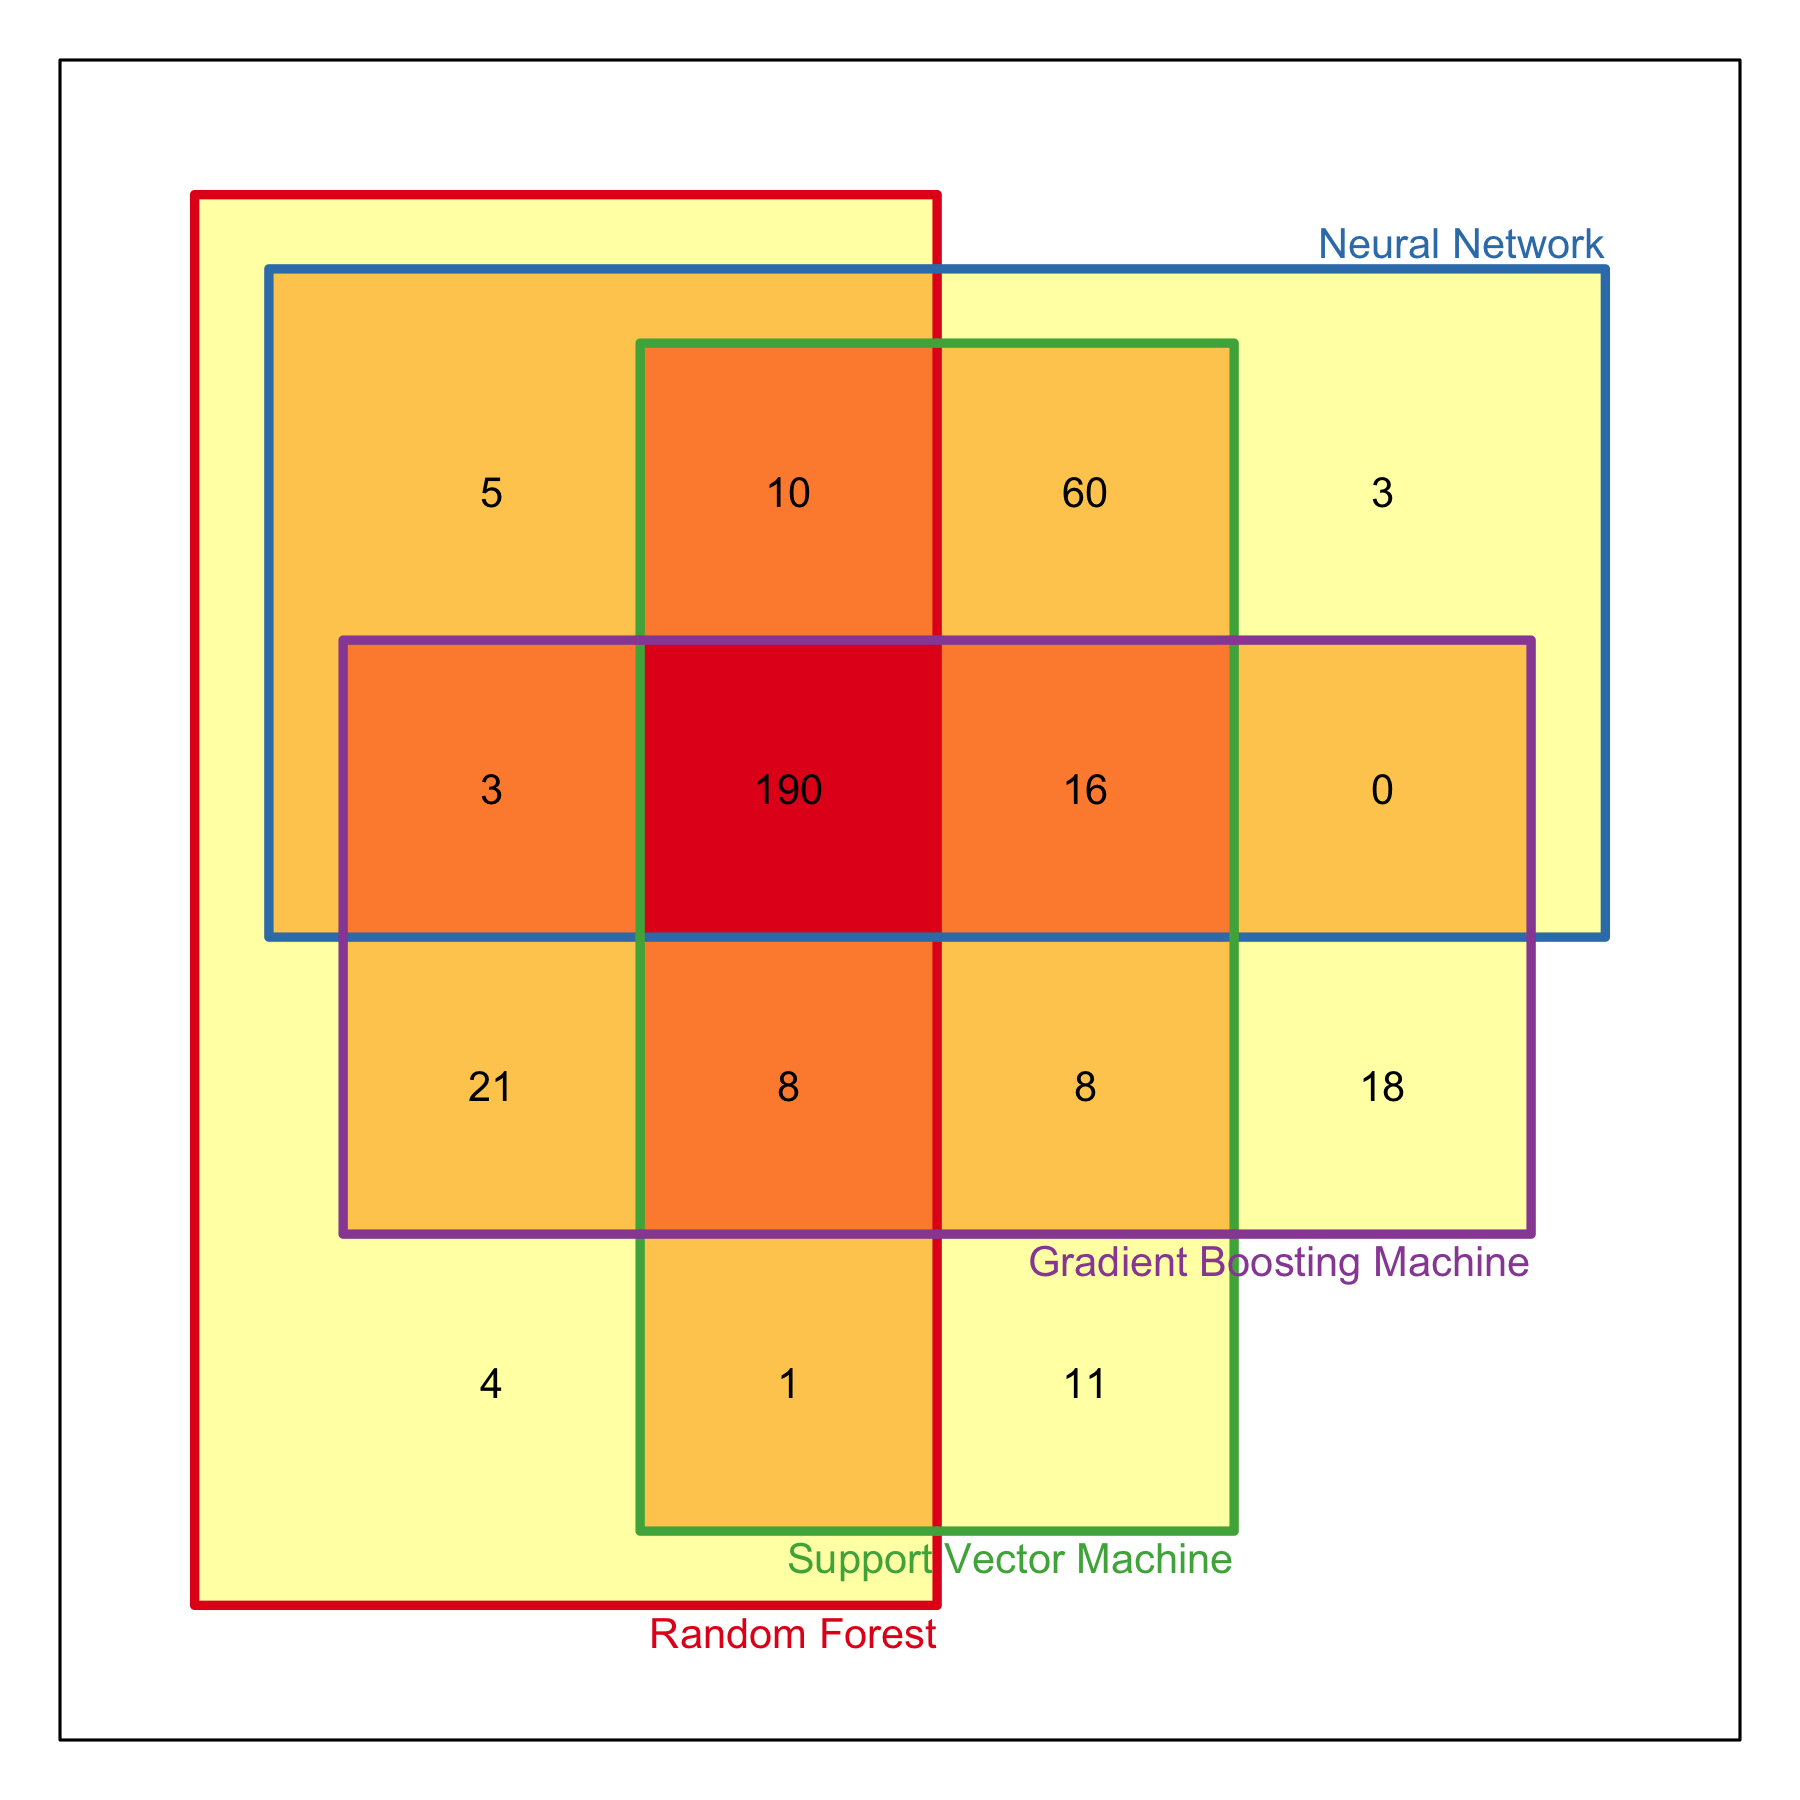
\includegraphics{pics/VennTargets.png}
    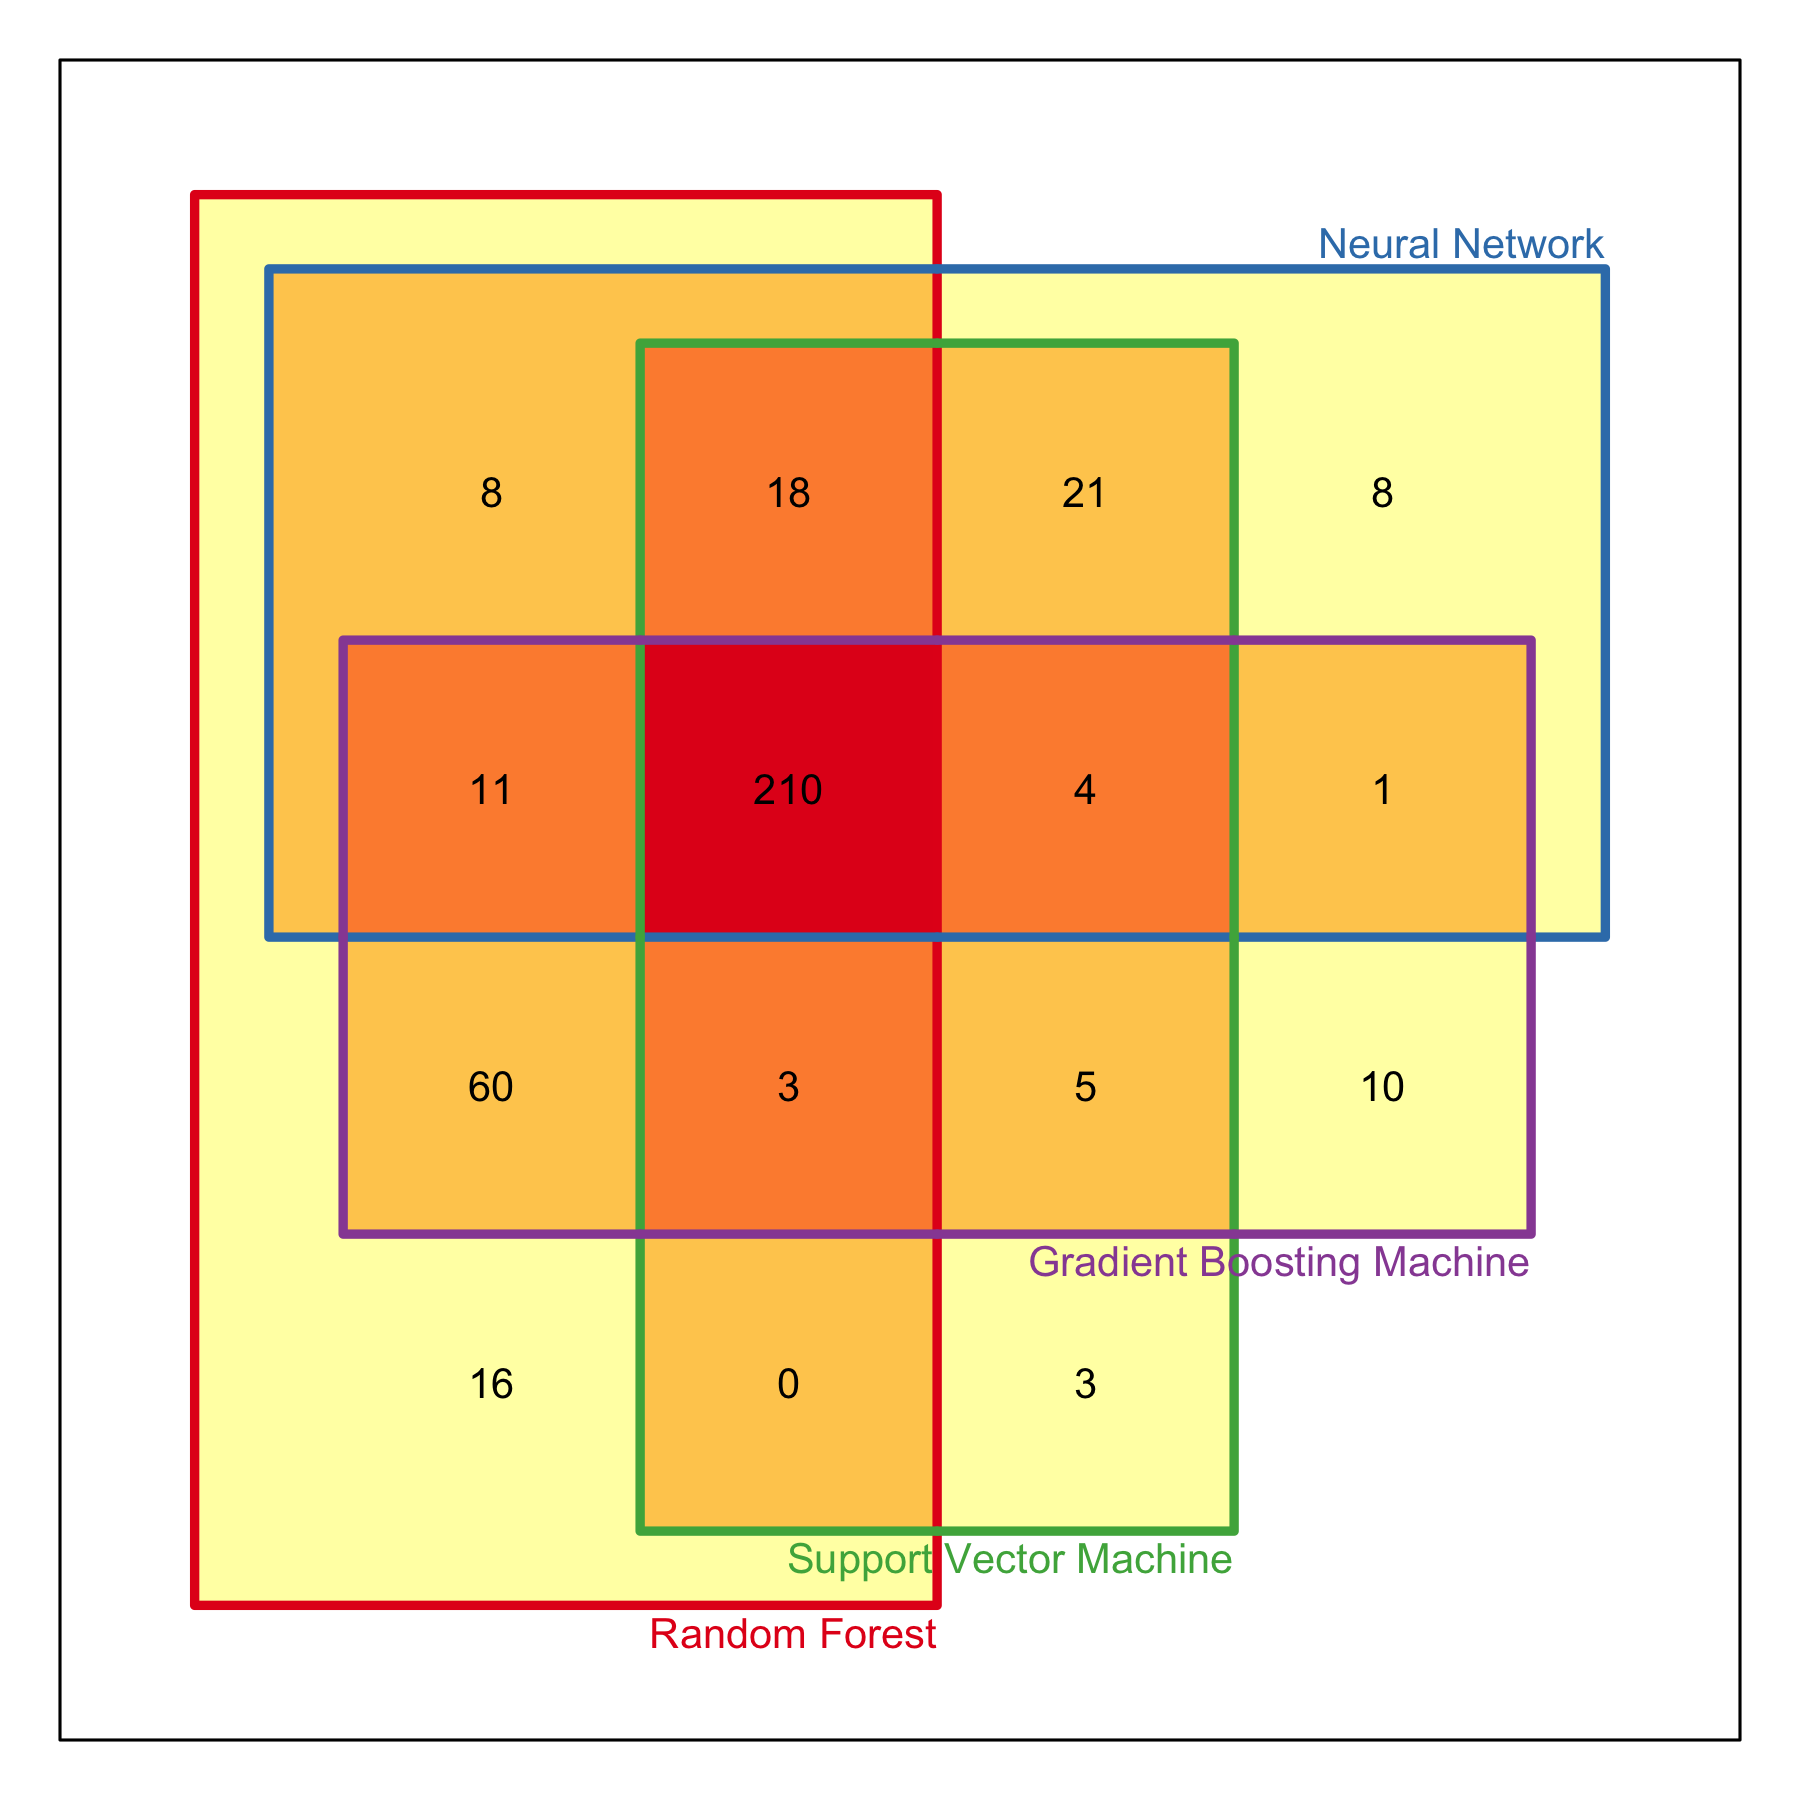
\includegraphics{pics/VennNontargets.png}}
    \caption{Overlap of predicted targets across the four trained classifiers. Venn diagrams showing the relative overlap of predicted targets (left) and predicted non-targets (right) from the \texttt{training set} for the four trained classifiers \label{fig:OT_venn}}
\end{figure}

To further ensure that they were not overfitting the models to the training data, they also evaluated the performances of the four classifiers on the \texttt{test set} (see Figure \ref{fig:ot_workflow}) that was not previously fed in the training of the binary classifiers. The performance of all four trained models was consistent with the NCV results on the \texttt{training set} in both Ferrero et al. \cite{ferrero2017} and my results (see Table \ref{tab:David_perf_train_mean}). This indicates that overfitting did not occur.

\begin{table}[H]
\centering
\begin{tabular}{c|c|c|c|c|c|c|c}
Classifier & MMCE  & Accuracy   & AUC   & Recall/Sensitivity   & Specificity   & Precision   & F1    \\
\hline
RF & 0.289 & 0.711 & 0.720 & 0.649 & 0.779 & 0.762 & 0.701 \\
NN & 0.296 & 0.704 & 0.698 & 0.730 & 0.676 & 0.711 & 0.720 \\
SVM & 0.303 & 0.697 & 0.722 & 0.743 & 0.647 & 0.696 & 0.719 \\
GBM & 0.373 & 0.627 & 0.664 & 0.622 & 0.632 & 0.648 & 0.634
\end{tabular}
\caption{\textbf{David results}. \texttt{Test set} performance measures (misclassification error, accuracy, AUC, recall/sensitivity ratio, specificity, precision, F1 measure) for all trained classifiers \label{tab:OT_perf_test}}
\end{table}

\subsubsection{TO DO}
\begin{itemize}
    \item Predicted targets in the \texttt{prediction set}
    \item Histograms for different stages or phases of development (Data from PharmaProjects)
    \item Literature text mining for validation (I do not have this data from Docstore)
\end{itemize}

An intrinsic limitation of validation methods for ML is the use of the same source of information as a label \cite{ferrero2017}. Ferrero et al. used \textbf{scientific literature} as an external source of information for the validation. Concretely, they mined co-occurrences of gene or proteins being flagged as potential therapeutic targets in titles and abstracts of published articles in MEDLINE \cite{ferrero2017}. They found 25,603 GDAs, corresponding to 4413 unique genes\cite{ferrero2017}. 590 of these 4413 genes were in common with the predicted targets by the trained NN model, a highly significant proportion as assessed by Fisher’s exact test (p = 5.05e−172, odds ratio = 5.78) \cite{ferrero2017}

\subsubsection{Limitations}
\label{subsub:limitations_openTargets}
\begin{itemize}
    \item \textbf{Labelling of the classes}: there is no pure negative nor positive class which complicates the problem of a binary classification: defining \emph{bona fide} unsuccessful targets is extremely difficult, if possible at all.
    
    Failed or abandoned projects according to Informa Pharmaprojects were ignored \cite{ferrero2017}. It is unclear the why the projects failed or were abandoned: (i) one target could be perfectly viable but it may have been withdrawn for commercial or R\&D reasons or (ii) unsuccessful targets in one area may be valuable in others.
    
    Ferrero et al. \cite{ferrero2017} assumed that the unlabelled, negative set contained both future positive targets, not being actively pursued as therapeutics, and negative targets for any reason. From an algorithmic perspective, they simply treated the unlabelled data as the negative set, allowing them to use supervised learning methods within a semi-supervised setting according to \cite{elkanUnlabelled2015}. Nonetheless, for this reason, (i) the number of true positives is going to be underestimated or, in other words, (ii) the false positive rate is overestimated, leading to worse precision and sensitivity/recall estimates \cite{ferrero2017}.
    
    Additionally, some drugs in early stages of drug development were defined as \emph{positive} successful targets but they may fail in latter stages.
    
    \item In terms of performance, the NN model was the best with a 71\% accuracy even though no classifier significantly outperformed the others. Nevertheless, this is not a great performance. Can I do better including more data types or using different ML algorithms?
    
    \item  Inclusion of functional (Gene Ontology, pathways), structural (protein domains) or interaction data (protein–-protein interactions) is likely to have a large impact on the ability to successfully predict therapeutic targets as it has been already demonstrated \cite{ferrero2017}. Ferrero et al. did not considered these data types.
    
    \item Their model correctly classified later stage drug targets more easily than earlier stages targets.  Therapeutic targets more advanced in the drug discovery pipeline show clearer differences and thus appear more straightforward to discriminate \cite{ferrero2017}.
    
    \item Their predictions were individual targets, and not target–-indication or target--disease pairs: they predicted potential therapeutic targets, regardless of the intended indication.
    
    \item Ferrero et al. did not make any claim regarding the druggability of these targets. Open Targets answers questions focused on GDAs but is unable to report focused aspects about the bioactivity profiles of small molecules on those targets \cite{brown2018}
    
    \item Ferrero et al. removed the feature \texttt{literature} since it it was likely to be heavily biased towards well known, validated target–indication pairs and, in addition, they used it to validate their approach. What about \texttt{animal\_model}?
    
    \item Why \texttt{animal\_model} is a good feature for predicting (like they say in the title!) \textbf{novel} therapeutics? Is not just a mere reflection of how much effort has been put on a given GDA? How much money has already been invested in deciphering a GDA? How much time has been spent or even lost in a GDA? How novel targets are going to have high scores in \texttt{animal\_models}? Ferrero et al. \cite{ferrero2017} reported that the algorithm was able to predict much better genes that had pharmaceutics in the market. Is not that obvious? Are not genes with human orthologs in animals been studied in clinical phases before being launched to the market?
    
    Stoeger and colleagues \cite{stoeger2018} demonstrated that the impact of research on model organisms particularly influenced research in human genes. Furthermore, Homologous genes of unstudied human genes are likewise unstudied in model organisms.
    
    Because if there is a high score in the \texttt{animal\_model} feature, it can mean to things: (i) the GDA is already well defined, well studied before doing the animal model and there is a target for it or (ii) the GDA has been a failure and there is no target yet.
\end{itemize}

Finally, Ferrero et al. \cite{ferrero2017} reported that they did not neglected inference. They report that their decision tree gains some insights into the characteristics that makes good therapeutic targets \cite{ferrero2017}. But, the main feature in the decision tree is \texttt{animal\_model}. How do they infer this? Where is the causality? How making an experiment in an animal converts a target in a good target? It just turns out that no one, surprisingly, is going to waste resources in experimenting with animals without enough evidences. What if we made animal experiments in all human ortholog genes? Would all these genes be good targets? Their research is just based on prediction! There is no causal inference anywhere.

Focusing on the publications reporting the discovery of new human genes, we found an overrepresentation of publications that cite studies of nonhuman genes (Figs 2D and S6A). Inspecting the organisms of these genes, we observed two classes of organisms. The first class preferentially co-occurred together with human genes and consisted of Mus musculus, Rattus norvegicus, Bos taurus, and Gallus gallus (37%, 9.1%, 2.6%, 2.5% of all citations, respectively). The second class preferentially occurred in publications without human genes and consisted of Drosophila melanogaster, Saccharomyces cerevisiae, Escherichia coli, Xenopus laevis, Caenorhabditis elegans, and Schizosaccharomyces pombe (22%, 10%, 4.0%, 2.5%, 1.6%, 1.5% of all citations, respectively) (S6B Fig). Assuming that citations are one proxy of scientific impact, this finding suggests that initial reports on human genes have been particularly influenced by research in model organisms and that multiple model organisms have contributed complementary roles in the discovery of human genes.

With these insights, we dramatically increased the prediction accuracy of the year of initial report of a human gene by including the years of the initial reports on homologous genes of model organisms (Fig 2E, from Spearman: 0.48 to 0.71). Moreover, the years of the initial reports on homologous genes improved prediction accuracy of the number of publications to a greater extent than the year of the initial report on the human genes themselves (S7A Fig, Spearman: 0.81).

Consistent with the picture emerging from these analyses, the homologous genes of unstudied human genes are likewise unstudied in model organisms (S6 Table), and including the number of publications on homologous genes yielded almost perfect predictions of the number of publications for individual human genes (Fig 2F, Spearman: 0.87), while human-specific genes without homologous genes remain significantly less studied (S7B Fig, Mann–Whitney U test: p-value < 10−32). Taken together, these findings demonstrate the impact of research on model organisms on the knowledge acquired on human biology—a hypothesis that had been proposed but not demonstrated previously [32].